
%Template pembuatan naskah skripsi.
\documentclass{jtetiskripsi}
\usepackage{geometry}
\usepackage{kantlipsum}
\usepackage{fancyhdr}
\usepackage{longtable}
\fancyhf{} % clear all header and footers
\renewcommand{\headrulewidth}{0pt} % remove the header rule
\fancyfoot[RO]{\thepage} % Left side on Even pages; Right side on Odd pages
\pagestyle{fancy}
\fancypagestyle{plain}{%
	\fancyhf{}%
	\renewcommand{\headrulewidth}{0pt}%
	\fancyhf[rof]{\thepage}%
}
%Untuk prefiks pada daftar gambar dan tabel
\usepackage[titles]{tocloft}
\renewcommand\cftfigpresnum{Gambar\  }
\renewcommand\cfttabpresnum{Tabel \   }

%Untuk hyperlink dan table of content
\usepackage{hyperref}
\newlength{\mylenf}
\settowidth{\mylenf}{\cftfigpresnum}
\setlength{\cftfignumwidth}{\dimexpr\mylenf+2em}
\setlength{\cfttabnumwidth}{\dimexpr\mylenf+2em}

%Untuk Bold Face pada Keterangan Gambar
\usepackage[labelfont=bf]{caption}

%Untuk caption dan subcaption
\usepackage[labelsep=none]{caption}
\usepackage{subcaption}


%-----------------------------------------------------------------
%Disini awal masukan untuk data proposal skripsi
%-----------------------------------------------------------------



%-----------------------------------------------------------------
%Disini akhir masukan untuk data proposal skripsi
%-----------------------------------------------------------------


\begin{document}

\cover

\approvalpage

%-----------------------------------------------------------------
%Disini awal masukan Acknowledment
%-----------------------------------------------------------------
\acknowledgment
\begin{flushright}
\emph{Untuk Ibu, Bapak,\\dan Adik-adikku tercinta.}
\end{flushright}

%-----------------------------------------------------------------
%Disini awal masukan untuk Prakata
%-----------------------------------------------------------------
\preface
Assalamu'alaikum Wr. Wb.

\vspace{0.5cm}

Puji syukur penulis panjatkan ke hadirat Allah SWT karena hanya dengan rahmat dan hidayah-Nya, Tugas Akhir ini dapat terselesaikan tanpa halangan berarti. Keberhasilan dalam menyusun laporan Tugas Akhir ini tidak lepas dari bantuan berbagai pihak yang mana dengan tulus dan ikhlas memberikan masukan guna sempurnanya Tugas Akhir ini. Oleh karena itu dalam kesempatan ini, dengan kerendahan hati penulis mengucapkan terima kasih kepada:

\begin{enumerate}

\item{Bapak Surya Michrandi Nasution, S.T., M.T Selaku Dosen Pembimbing pertama saya, dan sebagai KK Seculab }
\item{Bapak Fairuz Azmi, S.T., M.T Selaku Dosen Pembimbing kedua saya }
\item {Bapak Ir. Burhanuddin Dirgantoro ,M.T Selaku Dosen Wali saya}
\item{Temen-temen kelas SK-37-04 yang selalu membuat saya tertawa dengan humornya}

\item{Dan Teman-teman yang masih banyak yang tidak mungkin saya sebutkan}

\end{enumerate}

Penulis menyadari bahwa penyusunan Tugas Akhir ini jauh dari sempurna.Akhir kata penulis mohon maaf yang sebesar-besarnya apabila ada kekeliruan di dalam penulisan Tugas Akhir ini.

\vspace{0.5cm}

Wassalamu'alaikum Wr. Wb.

\begin{tabular}{p{7.5cm}c}
&Bandung, 28 Juni 2017\\
&\\
&\\
&\textbf{Penulis}
\end{tabular}

%-----------------------------------------------------------------
%Disini akhir masukan untuk muka skripsi
%-----------------------------------------------------------------
\tableofcontents
\addcontentsline{toc}{chapter}{DAFTAR ISI}
\listoftables
\addcontentsline{toc}{chapter}{DAFTAR TABEL}
\listoffigures
\addcontentsline{toc}{chapter}{DAFTAR GAMBAR}

%-----------------------------------------------------------------
%Daftar Singkatan [Optional]
%-----------------------------------------------------------------

%-----------------------------------------------------------------
%Disini awal masukan Intisari
%-----------------------------------------------------------------
\begin{abstractind}
Dalam perkembangan teknologi sekarang yang sudah semakin pesat, kebutuhan akan keamanan jaringan tentunya meningkat seiring dengan berkembangnya
ilmu pengetahuan tentang masalah hacking dan cracking yang bersifat free dan ada
pula yang dikomersilkan. Kemudian dari sisi software pendukung pun sudah banyak
tool-tool yang bersifat free yang kemampuannya sudah bisa dikatakan mumpuni untuk digunakan sebagai alat penyerangan oleh kalangan attacker.

Pada sisi lain timbul masalah serius yaitu faktor keamanannya, namun disatu
sisi manusia sudah sangat tergantung dengan sistem informasi. Hal itu yang menyebabkan statistik insiden keamanan jaringan terus meningkat tajam dari tahun ke tahun.
Ini disebabkan karena kepedulian masyarakat yang sangat kurang terhadap sistem
keamanan jaringan.


Pada permasalahan tersebut, pada penelitian ini akan dibuat sebuah aplikasi
yang dapat membantu network administrator dalam memonitoring server, aplikasi ini
bertujuan untuk mempermudah network administrator dalam mengamankan server
dari berbagai macam jenis serangan (ddos, scaning , brute force)

\bigskip
\noindent
\textbf{Kata kunci :} \emph{TelegramBot, attacker , server, ddos , scanning , brute force}
\end{abstractind}

\begin{abstracteng}
\emph { In today's rapidly growing technological developments, the need for network security certainly increases with the development of knowledge about hacking and cracking problems that are free and some are commercialized. Then from the side of the software support is already a lot of tool tools that are free of which ability can be said to be used as a means of attack by attackers.}
 
\emph{ On the other hand there is a serious problem that is the security factor, but on the one hand humans are very dependent with the information system. This is what causes the statistics of network security incidents continue to increase sharply from year to year. This is due to the people's awareness which is very less towards Network security system.}
 
\emph{ In this research, we will create an application that can help network administrator in monitoring server, this application is aimed to facilitate network administrator in securing server from various kinds of attack (ddos, scaning, brute force) }
 
\bigskip
\noindent
\textbf{\emph{Keywords :}} \emph{wireless sensor network, Internet Protokol, WiFi, interoperability}.
\end{abstracteng}
%-----------------------------------------------------------------
%Disini akhir masukan Intisari
%-----------------------------------------------------------------

%-----------------------------------------------------------------
%Disini awal masukan untuk Bab
%-----------------------------------------------------------------
%!TEX root = ./template-skripsi.tex
%-------------------------------------------------------------------------------
% 								BAB I
% 							LATAR BELAKANG
%-------------------------------------------------------------------------------

\chapter{LATAR BELAKANG}

\section{Latar Belakang Masalah}
Dalam perkembangan teknologi yang semakin pesat, kebutuhan akan keaman-
an jaringan tentunya meningkat seiring dengan berkembangnya ilmu pengetahuan
tentang masalah \emph{hacking} dan \emph{cracking} yang bersifat \emph{free} dan ada pula yang diko-
mersilkan. Kemudian dari sisi \emph{software} pendukung pun sudah banyak \emph{tools} yang
bersifat \emph{free} yang kemampuannya sudah bisa dikatakan mumpuni untuk digunakan
sebagai alat penyerangan oleh kalangan \emph{attacker}.

Pada sisi lain timbul masalah serius yaitu faktor keamanannya, namun disatu
sisi manusia sudah sangat tergantung dengan sistem informasi. Hal itu yang me-
nyebabkan statistik insiden keamanan jaringan terus meningkat tajam dari tahun ke
tahun. Ini disebabkan karena kepedulian masyarakat yang sangat kurang terhadap
sistem keamanan jaringan

Keamanan jaringan lokal ini bergantung sepenuhnya terhadap bagaimana se-
orang \emph{network administrator} merespon dengan cepat sebuah serangan yang terjadi.
Tapi \emph{network administrator} hanyalah seorang manusia yang terbatas akan waktu. Se-
orang \emph{network administrator} tidak dapat mengawasi seluruh jaringan secara terus-
menerus. Maka dari itu dibutuhkan sebuah sistem yang dapat membantu \emph{network
administrator} untuk digunakan sebagai mengetasi segala macam serangan.
Pada permasalahan tersebut, pada penelitian ini akan dibuat sebuah aplikasi
yang dapat membantu \emph{network administrator} dalam \emph{memonitoring server}, aplikasi ini
bertujuan untuk mempermudah \emph{network administrator} dalam mengamankan \emph{server}
dari berbagai macam jenis serangan \emph{(ddos, scaning , brute force)}.
 
Selain itu aplikasi ini terhubung dengan fitur bot yang dimiliki oleh aplika-
si \emph{chat} telegram, yang berfungsi sebagai \emph{command and control} pada server. Setiap
serangan yang terdeteksi akan dikirim melalui telegram, sehingga \emph{network adminis-
trator} dapat mengetahui serangan apa saja yang terjadi pada \emph{server} ditambah dengan
fitur bot dari telegram yang berfungsi sebagai \emph{command and control} yang digunakan
untuk memerintah \emph{server} untuk melakukan pencegahan / \emph{bloking}.

\section{Rumusan Masalah}
Dalam perkembangan teknologi sekarang yang sudah semakin pesat, kebu-
tuhan akan keamanan jaringan tentunya meningkat seiring dengan berkembangnya
ilmu pengetahuan tentang masalah \emph{hacking} dan \emph{cracking} yang bersifat free dan ada
pula yang dikomersilkan. Kemudian dari sisi software pendukung pun sudah banyak
tool-tool yang bersifat free yang kemampuannya sudah bisa dikatakan mumpuni un-
tuk digunakan sebagai alat penyerangan oleh kalangan attacker. Serangan-serangan
tersebut dapat melumpuhkan server. Sehingga dapat menimbulkan kerugian.


\section{Batasan Masalah}
Batasan masalah pada penelitian ini adalah:
\begin{enumerate}
\item Membutuhkan kapasitas memori yang cukup besar.
\item Berjalan sistem operasi linux .
\item Hanya bisa melakukan monitoring pada satu \emph{interface network} saja..
\item Hanya mendeteksi serangan (DDoS, Scanning, Brute Force)
\end{enumerate}

\section{Hipotesis}
Dengan menggunakan rule deteksi yang didapatkan dengan pengolahan data-
sheet akan ditemukan fitur serangan yang mempunyai ciri-ciri masing-masing dalam
jenis serangan, hal ini akan mempermudah dalam melakukan deteksi serangan ter-
sebut, dikarenakan semua jenis serangan akan dibedakan dari masing masing fitur
serangan yang telah ditentukan. Dalam mendeteksi serangan diharapkan sekurang-kurangnya 70\% 


\section{Tujuan Penelitian}
Tujuan dari penelitian tugas akhir ini adalah membuat sebuah aplikasi yang digunakan untuk membantu \emph{sysadmin} dalam memonitoring serangan-serangan yang terjadi pada \emph{server}, baik dalam proses pencegahan dan pendektesian terhadap serangan yang mempu membahayakan \emph{server}.



\section{Metode Penyelesain Masalah}

Metode penelitian yang digunakan:
\begin{enumerate}

\item  STUDI LITERATUR. \newline
Melakukan pencarian refrensi mengenai telegram bot dan pengolahan data tra-
fik jaringan berdasarkan serangan yang diperlukan.

\item PENGUMPULAN DATA. \newline
Pada tahap ini, dilakukan pengumpulan data training yang akan diolah meng-
gunakan algoritma Decision Tree. Data training dikumpulkan menggunakan
scapy. Data Training pada serangan DDoS, Brute Force dan Scanning masing-
masing berjumlah 5 juta data.

\item PERANCANGAN KEBUTUHAN SISTEM. \newline
Melakukan perancangan sistem deteksi untuk mendeteksi serangan DDoS, Bru-
te Force dan Scanning serta dapat di integrasikan terhadap library scapy


\item PENGUJIAN SISTEM. \newline
Pada tahap ini sistem yang telah dibangun akan diuji berdasarkan hasil analisa
dari algoritma decision tree yang menghasilkan fitur dan rules serangan..Hasil
dari pengujian tersebut, diantaranya adalah kemampuan sistem untuk mengha-
silkan tree berdasarkan jumlah data training yang ditentukan dan kemampuan
sistem untuk mendeteksi serangan berdasarkan fitur dan rules serangan yang di
inputkan kedalam sistem deteksi.

\item ANALISA HASIL PENGUJIAN. \newline
Pada tahap analisis hasil pengujian, dilakukan perbandingan trafik serangan
terhadap jumlah keseluruhan trafik. Hasil dari analisis tersebut, diantaranya
adalah akurasi untuk mendeteksi serangan.

\item PENYUSUNAN LAPORAN TUGAS AKHIR. \newline
Pada tahap ini semua data dan hasil dari penelitian akan dibuat menjadi sebuah
laporan dengan sistematika penulisan yang sesuai dengan ketentuan institusi.

\end{enumerate}
\newpage
\section{Sistematika Penulisan}
\noindent
\textbf{BAB I : PENDAHULUAN}

Pada bab ini dijelaskan latar belakang, rumusan masalah, batasan, tujuan,
manfaat, keaslian penelitian, dan sistematika penulisan.\\


\noindent
\textbf{BAB II : TINJAUAN PUSTAKA DAN LANDASAN TEORI}

Pada bab ini dijelaskan teori-teori dan penelitian terdahulu yang digunakan
sebagai acuan dan dasar dalam penelitian.\\

\noindent
\textbf{BAB III : METODOLOGI PENELITIAN}

Pada bab ini dijelaskan metode yang digunakan dalam penelitian meliputi
langkah kerja, pertanyaan penilitian, alat dan bahan, serta tahapan dan alur penelitian.\\

\noindent
\textbf{BAB IV : HASIL DAN PEMBAHASAN}

Pada bab ini dijelaskan hasil penelitian dan pembahasannya.\\

\noindent
\textbf{BAB V : KESIMPULAN DAN SARAN}

Pada bab ini ditulis kesimpulan akhir dari penelitian dan saran untuk pengem-
bangan penelitian selanjutnya.\\


% Baris ini digunakan untuk membantu dalam melakukan sitasi
% Karena diapit dengan comment, maka baris ini akan diabaikan
% oleh compiler LaTeX.
\begin{comment}
\bibliography{daftar-pustaka}
\end{comment}


%!TEX root = ./template-skripsi.tex
%-------------------------------------------------------------------------------
%                            BAB II
%               TINJAUAN PUSTAKA DAN DASAR TEORI
%-------------------------------------------------------------------------------

\chapter{TINJAUAN PUSTAKA DAN DASAR TEORI}                

\section{Telegram Bot}
Telegram adalah aplikasi pesan chatting yang memungkinkan pengguna untuk
mengirimkan pesan chatting rahasia yang dienkripsi end-to-end sebagai keamanan
tambahan. Selain itu telegram dilengkapi dengan fitur bot yang bersifat open source
yang dimana fitur ini sangat cocok digunakan dalam penelitian ini. pada penelitian
ini penulis menggunakan aplikasi telegram dikarenakan fitur bot telegram bisa digu-
nakan sebagai \emph{Command and Control (CNC)} pada \emph{server} , baik \emph{memonitoring server}
, monitoring serangan. Namun pada penelitian ini bot difungsikan sebagai Command
and Control pada server yaitu jika terjadi serangan apakah alamat ipaddres yang ter-
deteksi akan di blok atau tidak. Sehingga sysadmin tidak perlu melakukan remote
server untuk itu[2].

\section {\emph{Intrusion Detection System (IDS)}}
Menurut Chris Brenton (2003:289), Intrusion Detection System (IDS) ada-
lah sistem pendeteksian penyusupan yang dapat melakukan scanning log-log access
dan menganalisis karakteristik-karakteristik dari file-file untuk mengetahui apakah fi-
le tersebut telah diserang. Intrusion Detection System mampu mendeteksi aktivitas
yang mencurigakan dalam sebuah sistem atau jaringan.[1]

\indent
\subsection {\emph {Network Intrusion Detection System (\emph{NIDS})}}
\emph{Network Intrusion Detection System} adalah sistem pendeteksian penyusupan
\emph{network}. \emph{network Intrusion Detection System} memiliki fungsi untuk menganalisis
paket di sebuah \emph{network} dan mencoba untuk menentukan apakah seorang cracker
sedang mencoba untuk masuk ke dalam sebuah sistem atau menyebabkan sebuah
serangan Denial of Service (DOS)[2].

\subsection{\emph{Host Intrusion Detection System (\emph{HIDS})}}
\emph{Host Intrusion Detection System} adalah sistem pendeteksian penyusupan host.
Sama seperti \emph{NIDS}, sebuah \emph{HIDS} menganalisis lalu lintas \emph{network} yang dikirimkan
menuju dan dari sebuah mesin tunggal. Sebagian besar dari \emph{NIDS} komersial saat ini
biasanya memiliki suatu unsur \emph{HIDS}, dan sistem-sistem ini disebut hybrid IDS[2].

\subsection{\emph{System Integrity Verifier (SIV)}}
\emph{System Integrity Verifier} adalah alat untuk verifikasi integritas sistem. Melacak
file-file sistem yang kritikal dan memberitahukan kepada administrator pada saat file-
file tersebut diubah (biasanya oleh seorang cracker yang mencoba untuk mengganti
file yang valid dengan sebuah Trojan Horse). Contoh dari SIV adalah Tripwire[3].

\subsection{\emph{Log File Monitor (LFM)}}
Log File Monitor adalah alat yang digunakan untuk membaca log-log yang
dihasilkan oleh servis- servis \emph{network} yang mencari pola-pola serangan. Contoh dari
LFM adalah Swatch[3].

\section{\emph{Distributed Denial of Service (DDoS)}}
Rui Zhong et al.[4] \emph{Distributed Denial of Service (DDoS)} adalah jenis se-
rangan yang dilakukan secara masif dengan tujuan mengganggu hak akses pengguna
jaringan. DDoS merupakan serangan flooding trafik yang dilakukan dengan sengaja
untuk mengganggu QoS dari sistem jaringan yang bertujuan untuk membuat sumber
daya server habis. Serangan DDoS pada dasarnya sama dengan serangan DoS namun
serangan dilakukan dengan banyak sumber secara serentak. Untuk melancarkan se-
rangan DDoS, penyerang biasanya mengumpulkan pasukan dengan cara mengambil
alih komputer-komputer yang kemudian dijadikan zombie yang merupakan komputer
yang siap diperintah dan dikendalikan oleh botnet[2].

\newpage 
\section{\emph{Brute Force Attack}}
\emph{Brute Force attack} adalah serangan pada protokol jaringan yang bertujuan un-
tuk mendapat hak akses penuh dengan cara melakukan kegiatan penebakan username
dan password login dari sebuah service dengan menggunakan kombinasi username
dan password yang berbeda[4] 


\section{\emph{Scanning}}
\emph{Scanning Attack} adalah serangan yang bertujuan pada jaringan yang bertujuan
untuk menemukan port ataupun service yang terdapat pada sebuah host yang sedang
tersambung kedalam jaringan[5].Berikut akan dijelaskan macam-macam serangan
scanning:

\subsection{\emph{Host Discovery}}
Serangan \emph{Host Discovery} adalah jenis serangan scaning yang digunakan untuk
mengetahui junmlah host yang sedang aktip pada suatu jaringan[5]. Jenis serangan
ini mengirimkan packet icmp kesetiap alamat subnet pada sebauh jaringan.


\subsection{\emph{Port Detections}}
Jenis serangan scanning ini bertujuan untuk mengetahui port-port yang sedang
terbuka pada sebuah host yang telah ditentukan. Untuk menemukan port yang terbu-
ka serangan ini melakukan pengiriman paket tcp terhadap host yang sedanga aktip
dengan menargetkan port 1-65536.

\subsection{\emph{Service Scanning}}
Jenis serangan scanning ini adalah serangan yang akan mengetahui macam
macam service yang berjalan pada sebuah host yang menjalankan port tertentu.Serangan
ini melakukan scanning pada masing-masing port yang sedang berjalan dan akan me-
lakukan penyamaan signature pada software yang menjalankan port tersebut[5].

\newpage
\subsection{\emph{Host Detection}}
Serangan scanning ini bertujuan untuk mengetahui jenis sistem operasi yang
dijalankan. Serangan ini menargetkan port 443 (netbios) yang mempunyai signature
(ciri-ciri) tiap masing-masing host[6].

\subsection{\emph{Scapy}}
Scapy adalah suatu library yang dibangun menggunakan bahasa pemrogram-
an python dan sangat powerfull untuk memanipulasi paket yang ada pada jaringan.
Scapy mampu membuat dan memecah paket-paket dari berbagai jenis protocol yang
ada, mentransimikannya, menangkapnya, menerima permintaan dan menjawabnya,
dan banyak lagi. Scapy dapat digunakan untuk menangani macam-macam kegiat-
an yang berhubungan dengan \emph{network}ing, seperti kegiatan "scanning","tracerouting",
"attack" atau "\emph{network} discovery". Scapy juga dapat mengajarkan kita tentang semua
proses-proses dari suatu protocol.


% Baris ini digunakan untuk membantu dalam melakukan sitasi
% Karena diapit dengan comment, maka baris ini akan diabaikan
% oleh compiler LaTeX.
\begin{comment}
\bibliography{daftar-pustaka}
\end{comment}


%!TEX root = ./template-skripsi.tex
%-------------------------------------------------------------------------------
%                            BAB III
%               		METODOLOGI PENELITIAN
%-------------------------------------------------------------------------------

\chapter{METODOLOGI PENELITIAN}

\section{Gambaran Umum}
Pada perancangan sistem menjelaskan mengenai alur dari proses yang diker-
jakan pada tugas akhir ini. Penjelasan yang ada meliputi alur deteksi \emph{anomali} dan
hal-hal yang terkait untuk sistem deteksi \emph{anomali}. Pada penelitian tugas akhir meng-
ikuti alur sistem seperti gambar berikut:


\begin{figure}[H]
	\centering
	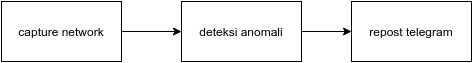
\includegraphics{gambar/gambaranUmum}
	\caption{Gambaran Umum Sistem}
	\label{Gambaran Umum Sistem}
\end{figure}

	\subsection{\emph{(Capture Network)}}
		Pada proses ini akan dilaukan monitoring \emph{traffik} menggunakan \emph{scappy} , setiap semua \emph{traffik} yang berjalan pada \emph{network} akan disamanakan dengan \emph{rule} deteksi yang sudah disediakan selama proses ini tidak akan dilakukan perintah apapun pada sisi \emph{server}. 
	\subsection{Deteksi \emph{Anomali}}
		Pada proses ini dilakukan pemindaian pada \emph{traffik} dan \emph{rule} deteksi yang digunakan, ketika \emph{traffik} tersebut sama dengan \emph{rule} serangan , maka akan terdeteksi sebagai anomali / serangan. Pada proses ini akan mengu perintah untuk melakukan bloking dari telegram.
		
	\subsection{Repost Telegram}
		Proses ini akan mengirim repost berupa pesan ,ketika terjadi anomali/serangan pada \emph{network} dan akan menunggu printah dari user untuk melakukan bloking dan sebagainya.
		
		
	
\section{Gambaran Khusus}


\begin{figure}[H]
	\centering
	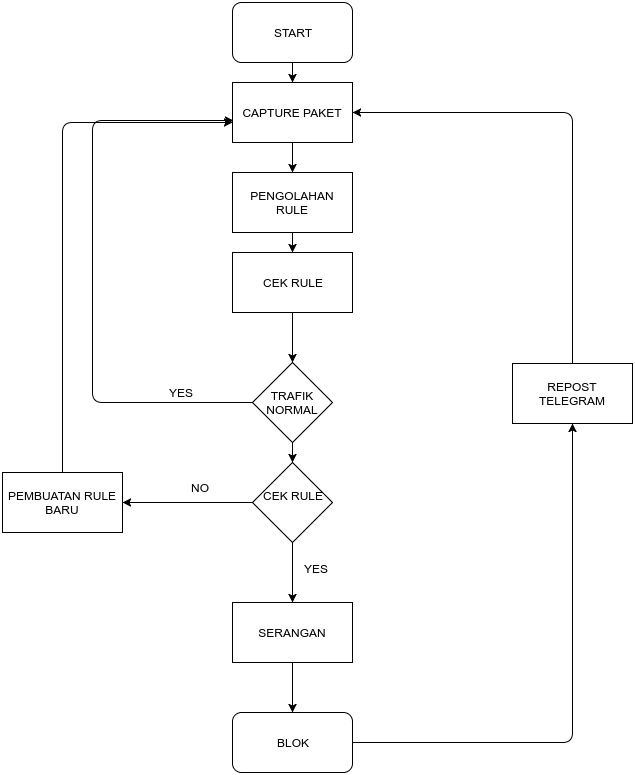
\includegraphics[scale = 0.9 ]{gambar/gambaranKhusus}
	\caption {Gambaran Khusus Sistem}
	\label{Gambaran Khusus Sistem }
\end{figure}

	\subsection{\emph{Capture Packet}}
	Pada proses ini akan dilaukan monitoring \emph{traffik} menggunakan \emph{scappy} , setiap semua \emph{traffik} yang berjalan pada \emph{network} akan disamanakan dengan \emph{rule} deteksi yang sudah disediakan selama proses ini tidak akan dilakukan perintah apapun pada sisi \emph{server}. 

	\subsection{Pengolahan \emph{Rule}}
	Proses ini akan melakukan pengolahan \emph{rule} yang digunakan untuk mendetesi serangan , setiap \emph{rule} yang terbentuk akan disimpan dalam sebuah file yang akan digunakan untuk deteksi anomali
	\subsection{Pemindain \emph{Rule}}
	Pada proses ini dilakukan pemindaian pada \emph{traffik} dan \emph{rule} deteksi yang digunakan, ketika \emph{traffik} tersebut sama dengan \emph{rule} serangan , maka akan terdeteksi sebagai anomali / serangan. Pada proses ini akan mengu perintah untuk melakukan bloking dari telegram.
	
	\subsection{\emph{Blocking}}
	Proses ini akan melakukan perintah dari user melalui telegram , pada proses ini blocking menggunakan tools iptables yang berfungsi sebagai tools untuk melakukan blok paket dan koneksi yang terhadi.
	
	\subsection{Repost Telegram}
	Proses ini akan mengirim repost berupa pesan ,ketika terjadi anomali/serangan pada \emph{network} dan akan menunggu printah dari dari user untuk melakukan bloking dan sebagainya.
	
	\subsection{Pembuatan \emph{Rule} Baru}
	Pada proses pembuatan \emph{rule} baru ini akan dilakukan ketika ada anommali dalam \emph{network} namum \emph{traffik} tersebut tidak terdeteksi sebagai serangan, sehingga dibutuhkan \emph{rule} baru untuk mendeteksi jenis \emph{traffik} tersebut.
\section{\emph{Capture Packet}}
Dalam Penelitian tugas akhir menggunakan fitur packet yang telah disesuaikan
dengan fitur pengoalahan \emph{rule} sebelumnya, yaitu dengan menggunakan dataset hasil
pengolahan dari capture scapy.

\section{Pengolahan \emph{Traffik}}
Pada pengoalahan trafik dilakukan proses pencocokan dengan hasil pengolah-
an dataset serangan yang telah didapatkan.

\begin{table}[H]
	\centering

	
	\caption{\ Jumlah dataset}
	\label{Jumlah dataset}
	\begin{tabular}{|c|l|l|}
		\hline
		NO & \emph{traffik}     & JUMLAH DATASET \\ \hline
		1  & SCANNING    & 5.000.000      \\ \hline
		2  & BRUTE FORCE & 5.000.000      \\ \hline
		3  & DDoS        & 5.000.000      \\ \hline
		4  & NORMAL      & 5.000.000      \\ \hline
	\end{tabular}
\end{table}

\section{Dataset}
Pada penelitian tugas akhir ini diguanakan dataset scapy. Berikut adalah fitur
dataset scapy antara lain:

	
\begin{enumerate}[A.]
	\begin{singlespace}
		\itemsep0em
		\item \emph{Transmission Control Protocol (TCP)}
		\item \emph{Internet Control Message Protocol (ICMP)}
		\item \emph{Internet Protocol Address (IP)}
		\item \emph{User Datagram Protocol (UDP)}

	\end{singlespace}
\end{enumerate}

berikut adalah penjelasan dari masing masing dataset yang digunakan untuk pembuatan \emph{rule} deteksi serangan .

	\newpage
	\subsection{\emph{Transmission Control Protocol (TCP)}}
	\emph{Transmission Control Protocol (TCP)} adalah suatu protokol yang berada di
	lapisan transport (baik itu dalam tujuh lapis model referensi OSI atau model DARPA)
	yang berorientasi sambungan (connection-oriented) dan dapat diandalkan (reliable).
	TCP dispesifikasikan dalam RFC 793.Pada scapy terdapat 11 fitur sebagai berikut : 
	
	\begin{table}[H]
		\centering
		\caption{\ Fitur ICMP}
		\label{Fitur ICMP}
		\begin{tabular}{|l|l|l|}
			\hline
			NO & FITUR     & TIPE \\ \hline
			1  & SPORT    & ShortEnumField      \\ \hline
			2  & DPORT & ShortEnumField      \\ \hline
			3  & SEQ        & IntField      \\ \hline
			4  & ACK      & IntField      \\ \hline
			5  & DATAOFS    & BitField      \\ \hline
			6  & RESERVED & BitField      \\ \hline
			7  & FLAGS        & FlagsField      \\ \hline
			8  & WINDOW      & ShortField     \\ \hline
			9  & CHKSUM    & XShortField      \\ \hline
			10  & ARGPTR &  ShortField      \\ \hline
			11  & OPTIONS        & TCPOptionsField      \\ \hline
		
		\end{tabular}
	\end{table}


	\newpage
	\subsection{\emph{Internet Control Message Protocol (ICMP)}}
	
	 Internet Control Message Protocol (ICMP) adalah salah satu protokol inti dari
	 keluarga protokol internet. ICMP utamanya digunakan oleh sistem operasi komputer
	 jaringan untuk mengirim pesan kesalahan yang menyatakan, sebagai contoh, bahwa
	 komputer tujuan tidak bisa dijangkau.
	 ICMP berbeda tujuan dengan TCP dan UDP dalam hal ICMP tidak digunak-
	 an secara langsung oleh aplikasi jaringan milik pengguna. salah satu pengecualian
	 adalah aplikasi ping yang mengirim pesan ICMP Echo Request (dan menerima Echo
	 Reply) untuk menentukan apakah komputer tujuan dapat dijangkau dan berapa lama
	 paket yang dikirimkan dibalas oleh komputer tujuan. Berikut adalah fitur icmp yang
	 terdapat pada scapy :
	 
	 
	 	\begin{table}[H]
	 	\centering
	 	\caption{\ Fitur ICMP}
	 	\label{Fitur ICMP}
	 	\begin{tabular}{|l|l|l|}
	 		\hline
	 		NO & FITUR     & TIPE \\ \hline
	 		1  & TYPE    & ByteEnumField      \\ \hline
	 		2  & CODE & MultiEnumField      \\ \hline
	 		3  & CHKSUM        & XShortField      \\ \hline
	 		4  & ID      & ConditionalField      \\ \hline
	 		5  & SEQ    & ConditionalField      \\ \hline
	 		6  & TSORI & ConditionalField      \\ \hline
	 		7  & TSRX        & ConditionalField      \\ \hline
	 		8  & TSTX      & ConditionalField     \\ \hline
	 		9  & GW    & ConditionalField      \\ \hline
	 		10  & PTR & ConditionalField      \\ \hline
	 		11  & RESERVED        & ConditionalField      \\ \hline
	 		12 & ADDRMASK	&  ConditionalField \\ \hline
	 		13 & UNUSED & ConditionalField \\ \hline
	 	\end{tabular}
	 	\end{table}
 	\newpage
 	\subsection{\emph{Internet Protocol Address (IP)}}
    	Internet Protocol Address (IP) adalah protokol lapisan jaringan (network la-
 	yer dalam OSI Reference Model) atau protokol lapisan internetwork (internetwork
 	layer dalam DARPA Reference Model) yang digunakan oleh protokol TCP/IP untuk
 	melakukan pengalamatan dan routing paket data antar host-host di jaringan kompu-
 	ter berbasis TCP/IP. Versi IP yang banyak digunakan adalah IP versi 4 (IPv4) yang
 	didefinisikan pada RFC 791 dan dipublikasikan pada tahun 1981, tetapi akan digan-
 	tikan oleh IP versi 6 pada beberapa waktu yang akan datang.Berikut adalah fitur yang
 	terdapat pada IP : 
 	
 	\begin{table}[H]
 		\centering
 		\caption{\ Fitur IP}
 		\label{Fitur IP}
 		\begin{tabular}{|l|l|l|}
 			\hline
 			NO & FITUR     & TIPE \\ \hline
 			1  & VERSION    & BitField      \\ \hline
 			2  & IHL & BitField      \\ \hline
 			3  & TOS        & XByteField      \\ \hline
 			4  & LEN      & ShortField      \\ \hline
 			5  & ID    & ShortField      \\ \hline
 			6  & FLAGS & FlagsField      \\ \hline
 			7  & FRAGS        & BitField      \\ \hline
 			8  & TTL      & ByteField     \\ \hline
 			9  & CHKSUM    & XShortField      \\ \hline
 			10  & SRC &  Emph      \\ \hline
 			11  & DST        & Emph      \\ \hline
 			12 & OPTIONS & PacketListField \\ \hline
 		\end{tabular}
 	\end{table}
 	
 	\subsection{\emph{User Datagram Protocol (UDP)}}
 	User Datagram Protocol merupakan bagian dari internet protocol. Dengan
 	UDP, aplikasi komputer dapat mengirimkan pesan kepada komputer lain dalam ja-
 	ringan lain tanpa melakukan komunikasi awal.[7]
 	UDP melakukan komunikasi secara sederhana dengan mekanisme yang sa-
 	ngat minimal. Ada proses checksum untuk menjaga integritas data. UDP digunakan
 	untuk komunikasi yang sederhana seperti \emph{query DNS (Domain Name System), NTP
 	 	(Network Time Protocol), DHCP (Dinamic Host Configuration Protocol), dan RIP
 	 	(Routing Information Protocol).}
 	

 
 

 \section{\emph{Autonomous System}}
 Cara kerja \emph{Autonomus System} ini adalah ketika \emph{traffik} terindikasi bukan \emph{traffik}
 normal, maka akan dilakukan pemindaian pada jenis serangan pada \emph{rule} yang telah
 disediakan, namun tidak semua \emph{rule} tersebut akan dianggap serangan. Pada kenyata-
 annya \emph{traffik} yang tidak terindikasi serangan ini merupakan serangan jenis lain yang
 dimana didalam \emph{rule} tersebut \emph{traffik} atau ciri ciri serangan ini belum ada. Oleh kere-
 na itu pada penelitian tugas akhir ini dibuat Autonomus System yang dimana \emph{traffik}
 serangan jenis baru secara langsung akan diolah menjadi \emph{rule} baru. Sehingga secara
 terus menerus akan mampu mengenali serangan tipe baru.
 Berikut adalah \emph{flowchart} Autonomus System :
 
 \begin{figure}[H]
 	\centering
 	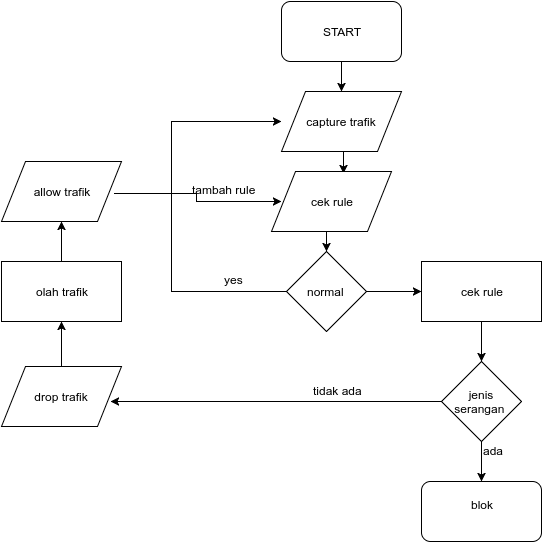
\includegraphics[scale = 0.8]{gambar/autonomusSystem}
 	\caption{Autonomous System}
 	\label{Autonomous System}
 \end{figure}
 
 
 
 \section{\emph{Telegram Command and Control (CNC)}}
 Telegram bot berfungsi sebagai \emph{Command and Control (CNC)} pada bagian ini
 aplikasi telegram berfungsi sebagai kimunikasi antara \emph{server} dan client. Ketika \emph{server}
 mendapat serangan , \emph{server} akan melakukan authentikasi melalui telegram ,sehingga
 sysadmin bisa melakukan tindakan defensive terhadap serangan tersebut berikut adalah gambar \emph{repost telegram}:
 
 
  \begin{figure}[H]
 	\centering
 	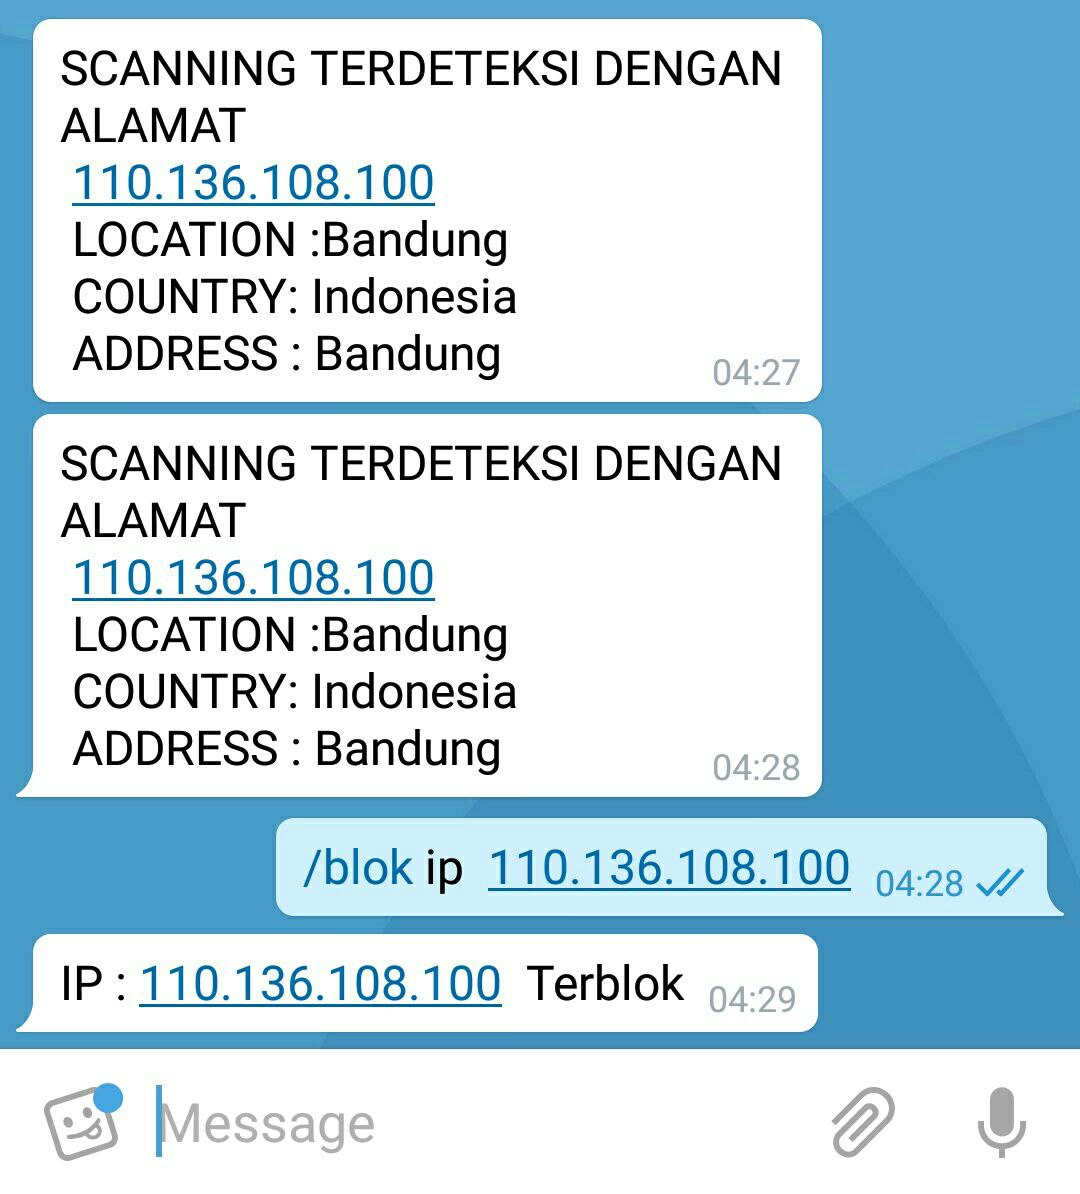
\includegraphics[scale = 0.15 ]{gambar/telegram_bot}
 	\caption{Telegram Repost}
 	\label{Telegram Repost}
 \end{figure}
 
  Berikut adalah \emph{flowchart} TelegramBot

 \begin{figure}[H]
	\centering
	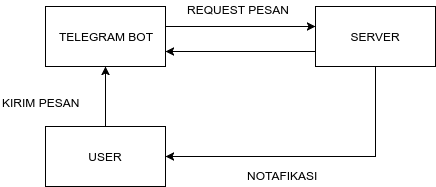
\includegraphics[scale = 0.7 ]{gambar/TELEGRAM}
	\caption{Telegram}
	\label{Telegram}
\end{figure}

Pada flowchrat diatas dapat deketahui \emph{user} mengirim pesan ketelegram , kemuadi setiap pesan akan dianggap sebuah perintah ketika pesan yang dikirimkan dikenali olah \emph{server} , setiap \emph{server} menerima serangan , pesan akan dikirim melalu telegram chat oleh bot ke user.
\section{\emph{Attacking Tools}}
Pada penelitian tugas akhir ini digunakan \emph{tools} untuk  melakukan \emph{attacking} sebagai berikut :


\subsection{NMAP}
\emph{NMAP (Network Mapper)} adalah sebuah aplikasi atau tool yang berfungsi untuk melakukan port \emph{scanning}. Aplikasi ini digunakan untuk meng-audit jaringan yang ada. Dengan menggunakan \emph{tools} ini, kita dapat melihat \emph{host} yang aktif, port yang terbuka, Sistem Operasi yang digunakan, dan \emph{feature-featur scanning} lainnya.

\subsection{NESSUS}
 
Nessus adalah scanner keamanan jaringan yang harus digunakan oleh administrator system . Nessus adalah software yang gratis dan bebas di download. Nessus merupakan sebuah software , yangdapat digunakan untuk meng-audit kemanan sebuah sistem, seperti vulnerability, misconfiguration,security patch yang belum diaplikasikan, default password, dan denial of service.

Nessus berfungsi untukmonitoring lalu-lintas jaringan.Dikarenakan fungsi dari Nessus dapat digunakan untuk mendeteksi adanya kelemahan ataupun cacatdari suatu sistem maka Nessus menjadi salah satu tool andalan ketika melakukan audit keamanan suatusistem. 

\subsection{METASPLOIT AUXILIARY}
Metasploit Auxiliary adalah sebuah tools yang diguanakan untuk melakukan penetrasi keamanan jaringan dengan memamfaatkan celah keaman yang ada , \emph{tools} ini suda dilengkapi dengan \emph{auxiliary} yang berfungsi sebagai tools tambahan untuk melakuan pemindaian pada jaringan yang bertujuan untuk menemukan celah pada jaringan sebelum diexploitasi.

\subsection{TCP Scanning}
Tools ini digunakan untuk melakukan pemindain pada sebuah jaringan yang bertujuan untuk mengetahui \emph{host} yang aktif dan tools ini juga bisa digunakan untuk melakukan pemindain \emph{port} pada \emph{host} yang aktip.

\subsection{HYDRA dan Medusa}
Hydra dan Medusa adalah sebuah tools yang didesain untuk melakukan \emph{brute force} pada sebuah \emph{service} yang membutuhkan \emph{authentication} berupa inputan login untuk dapat melaukan akses.

\subsection{Zero Brute}
Zero brute adalah sebauah tools yang digunakan untuk melakukan serangan \emph{brute force} yang bertujuan untuk mendapatkan hak akses secara penuh pada sebuah titik layanan.

\subsection{Metasploit SynFlood}
Metasploit Auxiliary adalah sebuah tools yang diguanakan untuk melakukan penetrasi keamanan jaringan dengan memamfaatkan celah keaman yang ada , \emph{tools} ini suda dilengkapi dengan \emph{auxiliary} yang berfungsi sebagai tools tambahan untuk melakuan pemindaian pada jaringan yang bertujuan untuk menemukan celah pada jaringan sebelum diexploitasi.

\subsection{Slowloris}
Slowloris adalah sebuah tools DDoS yang berfungsi sebagai alat untuk membanjiri lalu lintas jaringan sehingga bisa membuat layanan tidak bisa berfungsi dengan normal 

\subsection{HULK}
Tools ini didesain untuk membanjiri layanan HTTP dan HTTPS yang berfungsu sebagai titik layanan pada sebuah \emph{web server} , tool ini sering digunakan sebagai DDoS Bot

\subsection{PyLoris}
Tools ini hasil pengembangan dari \emph{slowloris} , tools ini bersifat open-source sehingga kita bisa mengatur layanan yang akan diserangan , biasanya tools ini diguanakan untuk menyerang layanan UDP .

\section{Alat dan Bahan}
	Alat dan bahan yang digunakan pada penelitian ini terbagi atas perangkat keras dan perangkat lunak yang akan dijelaskan seperti berikut.

	\subsection{Perangkat Keras}
	Adapaun perangakat keras yang kami gunakan pada peneletian kali ini adalah
	sebagai berikut

		\vspace{-0.5cm}

		\begin{enumerate}[a.]
		\begin{singlespace}
		\itemsep0em
			\item 1 buah server vps 
			\item 2 unit PC.
			\item 1 buah switch koneksi local (LAN)
			\item kabel LAN RJ45,
			\item 1 buah handphone,
		
		\end{singlespace}
		\end{enumerate}

	\subsection{Perangkat Lunak}
	Adapaun perangakat keras yang kami gunakan pada peneletian kali ini adalah
	sebagai berikut :

		\vspace{-0.5cm}

		\begin{enumerate}[a.]
		\begin{singlespace}
		\itemsep0em
			\item python compiler.
			\item module scapy.
			\item wireshark.
			\item mongodb.
			\item telegram.
			\item Linux Server.
			\item driffnet.
			\item etherape.
			\item nmap 
			\item metasploit 
			\item nessus 
			\item tcp scanning
	.
		\end{singlespace}
		\end{enumerate}


\begin{comment}
\bibliography{daftar-pustaka}
\end{comment}


%!TEX root = ./template-skripsi.tex
%-------------------------------------------------------------------------------
%                            BAB IV
%               		HASIL DAN PEMBAHASAN
%-------------------------------------------------------------------------------

\chapter{HASIL DAN PEMBAHASAN}

Pada penelitian tugas akhir ini, pengujian sistem deteksi \emph{anomali traffik} dila-
kukan dengan mengukur detection rate, accuracy. Data yang digunakan dalam pe-
ngujian berjumlah 5 juta dataset normal ,5 juta dataset serangan DDos ,5 juta dataset
serangan Brute Force ,5 juta dataset serangan Scanning. Pengujian pada peneltian
ini akan menghitung akurasi deteksi setiap serangan , kecepatan waktu komukiasin
antara server dan telegram, dan kapasitas memory yang digunakan oleh server dalam
menjalankan aplikasi ini.

	\section{Kebutuhan Pengujian}
		Data yang digunakan pada pengujian merupakan sebagian data dari dataset
		hasil scapy preprocessing yang telah telah dijadikan sebuah \emph{rule} dengan data seba-
		nyak masing masing 5 juta dataset . Data yang digunakan untuk proses training deci-
		sion tree menggunakan data dari hasil \emph{capturing traffik} menggunakan scapy dengan
		komposisi data yaitu data normal dan data serangan yang telah dijadikan \emph{rule} sebagai
		deteksi serangan. Pengujian ini menggunakan \emph{tools-tools} yang sudah bersifat umum dalam melakukan serangan dianataranta adalah sebagai berikut
		
		\subsection{\emph{Scanning Tools}}
		
		\vspace{-0.5cm}
		
		\begin{enumerate}[A.]
			\begin{singlespace}
				\itemsep0em
				\item NMAP
				\item NESSUS
				\item Metasploit auxilary
				\item TCP scanning tools,

				
			\end{singlespace}
		\end{enumerate}
		
			\subsection{\emph{Brute Force Tools}}
		
		\vspace{-0.5cm}
		
		\begin{enumerate}[A.]
			\begin{singlespace}
				\itemsep0em
				\item Hydra
				\item Medusa.
				\item Metasploit Auxiliary
				\item Zero brute
				\item Nmap Script Enggine 
				
			\end{singlespace}
		\end{enumerate}
	
		\subsection{\emph{DDoS Tools}}
	
	\vspace{-0.5cm}
	
	\begin{enumerate}[A.]
		\begin{singlespace}
			\itemsep0em
			\item Metasploit SynFlood
			\item Slowloris.
			\item TCP flood
			\item HULK (HTTP Unbearable Load King)
			\item PyLoris
			
		\end{singlespace}
	\end{enumerate}
\section{Pengujian Akurasi Masing-Masing Tools}
Pada pengujian ini akan diuji akurasi deteksi serangan dari masing masing \emph{tools} serangan yang digunakan dengan 10 kali percobaan terhadap 3 \emph{rule} serangan  , berikut adalah tabel pengujian serangan 

\subsection{NMAP}
Hasil akurasi deteksi NMAP dari 10 kali percobaan
\begin{table}[H]
	\centering
	\caption{Akurasi Deteksi Nmap}
	\label{Akurasi Deteksi Nmap}
	\begin{tabular}{|c|l|l|l|}
		\hline
		\multicolumn{1}{|l|}{Nomer}     & Scanning & Brute Force & DDoS   \\ \hline
		1                               & 93.00\%  & 5.00\%      & 0.00\% \\ \hline
		2                               & 94.00\%  & 6.00\%      & 0.00\% \\ \hline
		3                               & 94.00\%  & 6.00\%      & 0.00\% \\ \hline
		4                               & 93.00\%  & 5.00\%      & 0.00\% \\ \hline
		5                               & 94.00\%  & 6.00\%      & 0.00\% \\ \hline
		6                               & 94.00\%  & 6.00\%      & 0.00\% \\ \hline
		7                               & 92.00\%  & 8.00\%      & 0.00\% \\ \hline
		8                               & 94.00\%  & 6.00\%      & 0.00\% \\ \hline
		9                               & 94.00\%  & 6.00\%      & 0.00\% \\ \hline
		10                              & 94.00\%  & 6.00\%      & 0.00\% \\ \hline
		\multicolumn{1}{|l|}{rata-rata} & 93.60\%  & 6.33\%      & 0.00\% \\ \hline
	\end{tabular}
\end{table}
\newpage

\subsection{NESSUS}
Hasil akurasi deteksi NESSUS dari 10 kali percobaan
		\begin{table}[H]
			\centering
			\caption{Akurasi Deteksi Nessus}
			\label{Akurasi Deteksi Nessus}
			\begin{tabular}{|c|l|l|l|}
				\hline
				\multicolumn{1}{|l|}{Nomer}     & Scanning & Brute Force & DDoS   \\ \hline
				1                               & 91.00\%  & 6.00\%      & 0.00\% \\ \hline
				2                               & 92.00\%  & 6.00\%      & 0.00\% \\ \hline
				3                               & 90.00\%  & 8.00\%      & 0.00\% \\ \hline
				4                               & 88.00\%  & 8.00\%      & 0.00\% \\ \hline
				5                               & 90.00\%  & 6.00\%      & 0.00\% \\ \hline
				6                               & 94.00\%  & 6.00\%      & 0.00\% \\ \hline
				7                               & 94.00\%  & 6.00\%      & 0.00\% \\ \hline
				8                               & 95.00\%  & 5.00\%      & 0.00\% \\ \hline
				9                               & 95.00\%  & 5.00\%      & 0.00\% \\ \hline
				10                              & 96.00\%  & 4.00\%      & 0.00\% \\ \hline
				\multicolumn{1}{|l|}{rata-rata} & 92.50\%  & 6.00\%      & 0.00\% \\ \hline
			\end{tabular}
		\end{table}
	
\subsection{Metasploit Auxiliary}

Hasil akurasi deteksi \emph{Metasploit Auxiliary} dari 10 kali percobaan
\begin{table}[H]
	\centering
	\caption{Akurasi Deteksi Metasploit Auxiliary}
	\label{Akurasi Deteksi Metasploit Auxiliary}
	\begin{tabular}{|c|l|l|l|}
		\hline
		\multicolumn{1}{|l|}{Nomer}     & Scanning & Brute Force & DDoS   \\ \hline
		1                               & 90.00\%  & 8.00\%      & 0.00\% \\ \hline
		2                               & 91.00\%  & 6.00\%      & 0.00\% \\ \hline
		3                               & 92.00\%  & 6.00\%      & 0.00\% \\ \hline
		4                               & 90.00\%  & 8.00\%      & 0.00\% \\ \hline
		5                               & 91.00\%  & 6.00\%      & 0.00\% \\ \hline
		6                               & 94.00\%  & 6.00\%      & 0.00\% \\ \hline
		7                               & 92.00\%  & 8.00\%      & 0.00\% \\ \hline
		8                               & 94.00\%  & 6.00\%      & 0.00\% \\ \hline
		9                               & 94.00\%  & 6.00\%      & 0.00\% \\ \hline
		10                              & 98.00\%  & 2.00\%      & 0.00\% \\ \hline
		\multicolumn{1}{|l|}{rata-rata} & 92.60\%  & 6.20\%      & 0.00\% \\ \hline
	\end{tabular}
\end{table}

\subsection{TCP Scanning Tools}
Hasil Akurasi Deteksi \emph{TCP Scanning Tools} dari 10 kali percobaan 
\begin{table}[H]
	\centering
	\caption{Akurasi Deteksi TCP Scanning Tools}
	\label{Akurasi Deteksi TCP Scanning Tools}
	\begin{tabular}{|c|l|l|l|}
		\hline
		\multicolumn{1}{|l|}{Nomer}     & Scanning & Brute Force & DDoS   \\ \hline
		1                               & 98.00\%  & 2.00\%      & 0.00\% \\ \hline
		2                               & 94.00\%  & 6.00\%      & 0.00\% \\ \hline
		3                               & 92.00\%  & 8.00\%      & 0.00\% \\ \hline
		4                               & 94.00\%  & 6.00\%      & 0.00\% \\ \hline
		5                               & 94.00\%  & 6.00\%      & 0.00\% \\ \hline
		6                               & 98.00\%  & 2.00\%      & 0.00\% \\ \hline
		7                               & 94.00\%  & 6.00\%      & 0.00\% \\ \hline
		8                               & 94.00\%  & 6.00\%      & 0.00\% \\ \hline
		9                               & 95.00\%  & 5.00\%      & 0.00\% \\ \hline
		10                              & 95.00\%  & 5.00\%      & 0.00\% \\ \hline
		\multicolumn{1}{|l|}{rata-rata} & 94.80\%  & 5.20\%      & 0.00\% \\ \hline
	\end{tabular}
\end{table}


\subsection{Hydra}
Hasil akurasi deteksi hyrda dari 10 kali percobaan 

\begin{table}[H]
	\centering
	\caption{Akurasi Deteksi Hydra}
	\label{Akurasi Deteksi Hydra}
	\begin{tabular}{|c|l|l|l|}
		\hline
		\multicolumn{1}{|l|}{Nomer}     & Scanning & Brute Force & DDoS   \\ \hline
		1                               & 7.00\%   & 87.00\%     & 0.00\% \\ \hline
		2                               & 6.00\%   & 86.00\%     & 0.00\% \\ \hline
		3                               & 7.00\%   & 87.00\%     & 0.00\% \\ \hline
		4                               & 7.00\%   & 87.00\%     & 0.00\% \\ \hline
		5                               & 6.00\%   & 86.00\%     & 0.00\% \\ \hline
		6                               & 6.00\%   & 88.00\%     & 0.00\% \\ \hline
		7                               & 6.00\%   & 87.00\%     & 0.00\% \\ \hline
		8                               & 7.00\%   & 88.00\%     & 0.00\% \\ \hline
		9                               & 7.00\%   & 87.00\%     & 0.00\% \\ \hline
		10                              & 6.00\%   & 88.00\%     & 0.00\% \\ \hline
		\multicolumn{1}{|l|}{rata-rata} & 6.50\%   & 87.10\%     & 0.00\% \\ \hline
	\end{tabular}
\end{table}

\subsection{Medusa}
Hasil akurasi deteksi Medusa dari 10 kali percobaan
\begin{table}[H]
	\centering
	\caption{Akurasi deteksi medusa}
	\label{Akurasi deteksi medusa}
	\begin{tabular}{|c|l|l|l|}
		\hline
		\multicolumn{1}{|l|}{Nomer}     & Scanning & Brute Force & DDoS   \\ \hline
		1                               & 6.00\%   & 94.00\%     & 0.00\% \\ \hline
		2                               & 7.00\%   & 93.00\%     & 0.00\% \\ \hline
		3                               & 6.00\%   & 94.00\%     & 0.00\% \\ \hline
		4                               & 6.89\%   & 93.11\%     & 0.00\% \\ \hline
		5                               & 7.00\%   & 93.00\%     & 0.00\% \\ \hline
		6                               & 6.00\%   & 94.00\%     & 0.00\% \\ \hline
		7                               & 6.00\%   & 94.00\%     & 0.00\% \\ \hline
		8                               & 7.00\%   & 93.00\%     & 0.00\% \\ \hline
		9                               & 6.00\%   & 94.00\%     & 0.00\% \\ \hline
		10                              & 6.89\%   & 93.11\%     & 0.00\% \\ \hline
		\multicolumn{1}{|l|}{rata-rata} & 6.48\%   & 93.52\%     & 0.00\% \\ \hline
	\end{tabular}
\end{table}

\subsection{Metasploit Auxiliary}
Hasil akurasi Metasploit Auxiliary dari 10 kali percobaan

\begin{table}[H]
	\centering
	\caption{Akurasi Deteksi Metasploit Auxiliary}
	\label{Akurasi Deteksi Metasploit Auxiliary}
	\begin{tabular}{|c|l|l|l|}
		\hline
		\multicolumn{1}{|l|}{Nomer}     & Scanning & Brute Force & DDoS   \\ \hline
		1                               & 6.00\%   & 86.00\%     & 0.00\% \\ \hline
		2                               & 7.00\%   & 87.00\%     & 0.00\% \\ \hline
		3                               & 7.00\%   & 87.00\%     & 0.00\% \\ \hline
		4                               & 6.00\%   & 86.00\%     & 0.00\% \\ \hline
		5                               & 6.00\%   & 88.00\%     & 0.00\% \\ \hline
		6                               & 6.00\%   & 87.00\%     & 0.00\% \\ \hline
		7                               & 7.00\%   & 88.00\%     & 0.00\% \\ \hline
		8                               & 7.00\%   & 87.00\%     & 0.00\% \\ \hline
		9                               & 7.00\%   & 87.00\%     & 0.00\% \\ \hline
		10                              & 6.00\%   & 86.00\%     & 0.00\% \\ \hline
		\multicolumn{1}{|l|}{rata-rata} & 6.50\%   & 86.90\%     & 0.00\% \\ \hline
	\end{tabular}
\end{table}

\subsection{Zero Brute}
Hasil akurasi deteksi Zero Brute dari 10 kali percobaan
\begin{table}[H]
	\centering
	\caption{Akurasi deteksi Zero brute}
	\label{my-label}
	\begin{tabular}{|c|l|l|l|}
		\hline
		\multicolumn{1}{|l|}{Nomer}     & Scanning & Brute Force & DDoS   \\ \hline
		1                               & 6.00\%   & 87.00\%     & 0.00\% \\ \hline
		2                               & 7.00\%   & 88.00\%     & 0.00\% \\ \hline
		3                               & 7.00\%   & 87.00\%     & 0.00\% \\ \hline
		4                               & 7.00\%   & 87.00\%     & 0.00\% \\ \hline
		5                               & 6.00\%   & 86.00\%     & 0.00\% \\ \hline
		6                               & 6.00\%   & 88.00\%     & 0.00\% \\ \hline
		7                               & 6.00\%   & 87.00\%     & 0.00\% \\ \hline
		8                               & 7.00\%   & 88.00\%     & 0.00\% \\ \hline
		9                               & 7.00\%   & 87.00\%     & 0.00\% \\ \hline
		10                              & 7.00\%   & 87.00\%     & 0.00\% \\ \hline
		\multicolumn{1}{|l|}{rata-rata} & 6.60\%   & 87.20\%     & 0.00\% \\ \hline
	\end{tabular}
\end{table}

\subsection{Nmap Script Enggine}
Hasil akurasi deteksi Nmap Script Enggine dari 10 kali percobaan
\begin{table}[H]
	\centering
	\caption{Akurasi Nmap SCript Enggine}
	\label{Akurasi Nmap SCript Enggine}
	\begin{tabular}{|c|l|l|l|}
		\hline
		\multicolumn{1}{|l|}{Nomer}     & Scanning & Brute Force & DDoS   \\ \hline
		1                               & 7.00\%   & 87.00\%     & 0.00\% \\ \hline
		2                               & 6.00\%   & 86.00\%     & 0.00\% \\ \hline
		3                               & 6.00\%   & 88.00\%     & 0.00\% \\ \hline
		4                               & 6.00\%   & 87.00\%     & 0.00\% \\ \hline
		5                               & 7.00\%   & 88.00\%     & 0.00\% \\ \hline
		6                               & 7.00\%   & 93.00\%     & 0.00\% \\ \hline
		7                               & 6.00\%   & 94.00\%     & 0.00\% \\ \hline
		8                               & 6.89\%   & 93.11\%     & 0.00\% \\ \hline
		9                               & 7.00\%   & 93.00\%     & 0.00\% \\ \hline
		10                              & 6.00\%   & 94.00\%     & 0.00\% \\ \hline
		\multicolumn{1}{|l|}{rata-rata} & 6.49\%   & 90.31\%     & 0.00\% \\ \hline
	\end{tabular}
\end{table}

\subsection{Metasploit SynFlood}
Hasil akurasi deteksi Metasploit Synflood Enggine dari 10 kali percobaan
\begin{table}[H]
	\centering
	\caption{Akurasi Metasploit SynFlood}
	\label{Akurasi Metasploit SynFlood}
	\begin{tabular}{|c|l|l|l|}
		\hline
		\multicolumn{1}{|l|}{Nomer}     & Scanning & Brute Force & DDoS    \\ \hline
		1                               & 3.00\%   & 0.00\%      & 96.00\% \\ \hline
		2                               & 2.00\%   & 0.00\%      & 98.00\% \\ \hline
		3                               & 2.00\%   & 0.00\%      & 98.00\% \\ \hline
		4                               & 2.00\%   & 0.00\%      & 98.00\% \\ \hline
		5                               & 2.00\%   & 0.00\%      & 98.00\% \\ \hline
		6                               & 2.00\%   & 0.00\%      & 98.00\% \\ \hline
		7                               & 2.00\%   & 0.00\%      & 98.00\% \\ \hline
		8                               & 3.00\%   & 0.00\%      & 97.00\% \\ \hline
		9                               & 2.00\%   & 0.00\%      & 98.00\% \\ \hline
		10                              & 2.00\%   & 0.00\%      & 98.00\% \\ \hline
		\multicolumn{1}{|l|}{rata-rata} & 2.50\%   & 0.00\%      & 97.00\% \\ \hline
	\end{tabular}
\end{table}


\subsection{Slowloris}
Hasil akurasi deteksi slowloris dari 10 kali percobaan
\begin{table}[H]
	\centering
	\caption{Akurasi Deteksi Slowloris}
	\label{Akurasi Deteksi Slowloris}
	\begin{tabular}{|c|l|l|l|}
		\hline
		\multicolumn{1}{|l|}{Nomer}     & Scanning & Brute Force & DDoS    \\ \hline
		1                               & 3.00\%   & 0.00\%      & 96.00\% \\ \hline
		2                               & 2.00\%   & 0.00\%      & 98.00\% \\ \hline
		3                               & 2.00\%   & 0.00\%      & 98.00\% \\ \hline
		4                               & 2.00\%   & 0.00\%      & 98.00\% \\ \hline
		5                               & 2.00\%   & 0.00\%      & 98.00\% \\ \hline
		6                               & 2.00\%   & 0.00\%      & 98.00\% \\ \hline
		7                               & 2.00\%   & 0.00\%      & 98.00\% \\ \hline
		8                               & 3.00\%   & 0.00\%      & 97.00\% \\ \hline
		9                               & 2.00\%   & 0.00\%      & 98.00\% \\ \hline
		10                              & 2.00\%   & 0.00\%      & 98.00\% \\ \hline
		\multicolumn{1}{|l|}{rata-rata} & 2.50\%   & 0.00\%      & 97.00\% \\ \hline
	\end{tabular}
\end{table}


\subsection{TCP Flood}
Hasil akurasi deteksi TCP flood dari 10 kali percobaan
\begin{table}[H]
	\centering
	\caption{Pengujian Akurasi TCP Flood}
	\label{Pengujian Akurasi TCP Flood}
	\begin{tabular}{|c|l|l|l|}
		\hline
		\multicolumn{1}{|l|}{Nomer}     & Scanning & Brute Force & DDoS    \\ \hline
		1                               & 2.00\%   & 0.00\%      & 98.00\% \\ \hline
		2                               & 2.00\%   & 0.00\%      & 98.00\% \\ \hline
		3                               & 2.00\%   & 0.00\%      & 98.00\% \\ \hline
		4                               & 2.00\%   & 0.00\%      & 98.00\% \\ \hline
		5                               & 3.00\%   & 0.00\%      & 97.00\% \\ \hline
		6                               & 2.00\%   & 0.00\%      & 98.00\% \\ \hline
		7                               & 2.00\%   & 0.00\%      & 98.00\% \\ \hline
		8                               & 3.00\%   & 0.00\%      & 97.00\% \\ \hline
		9                               & 2.00\%   & 0.00\%      & 96.00\% \\ \hline
		10                              & 2.00\%   & 0.00\%      & 98.00\% \\ \hline
		\multicolumn{1}{|l|}{rata-rata} & 2.00\%   & 0.00\%      & 98.00\% \\ \hline
	\end{tabular}
\end{table}

\subsection{HULK}
Hasil akurasi deteksi Hulk dari 10 kali percobaan
\begin{table}[H]
	\centering
	\caption{Akurasi HULK}
	\label{Akurasi HULK}
	\begin{tabular}{|c|l|l|l|}
		\hline
		\multicolumn{1}{|l|}{Nomer}     & Scanning & Brute Force & DDoS    \\ \hline
		1                               & 3.00\%   & 0.00\%      & 96.00\% \\ \hline
		2                               & 2.00\%   & 0.00\%      & 98.00\% \\ \hline
		3                               & 2.00\%   & 0.00\%      & 98.00\% \\ \hline
		4                               & 2.00\%   & 0.00\%      & 98.00\% \\ \hline
		5                               & 2.00\%   & 0.00\%      & 98.00\% \\ \hline
		6                               & 2.00\%   & 0.00\%      & 98.00\% \\ \hline
		7                               & 2.00\%   & 0.00\%      & 98.00\% \\ \hline
		8                               & 3.00\%   & 0.00\%      & 97.00\% \\ \hline
		9                               & 2.00\%   & 0.00\%      & 98.00\% \\ \hline
		10                              & 2.00\%   & 0.00\%      & 98.00\% \\ \hline
		\multicolumn{1}{|l|}{rata-rata} & 2.50\%   & 0.00\%      & 97.00\% \\ \hline
	\end{tabular}
\end{table}


\subsection{PyLoris}
Hasil akurasi deteksi Pyloris dari 10 kali percobaan
\begin{table}[H]
	\centering
	\caption{Akurasi Deteksi Pyloris}
	\label{Akurasi Deteksi Pyloris}
	\begin{tabular}{|c|l|l|l|}
		\hline
		\multicolumn{1}{|l|}{Nomer}     & Scanning & Brute Force & DDoS    \\ \hline
		1                               & 2.00\%   & 0.00\%      & 98.00\% \\ \hline
		2                               & 2.00\%   & 0.00\%      & 98.00\% \\ \hline
		3                               & 2.00\%   & 0.00\%      & 98.00\% \\ \hline
		4                               & 2.00\%   & 0.00\%      & 98.00\% \\ \hline
		5                               & 3.00\%   & 0.00\%      & 97.00\% \\ \hline
		6                               & 2.00\%   & 0.00\%      & 98.00\% \\ \hline
		7                               & 2.00\%   & 0.00\%      & 98.00\% \\ \hline
		8                               & 3.00\%   & 0.00\%      & 97.00\% \\ \hline
		9                               & 2.00\%   & 0.00\%      & 96.00\% \\ \hline
		10                              & 2.00\%   & 0.00\%      & 98.00\% \\ \hline
		\multicolumn{1}{|l|}{rata-rata} & 2.00\%   & 0.00\%      & 98.00\% \\ \hline
	\end{tabular}
\end{table}
	\section{Pengujian Akurasi}		
		Pada pengujian ini untuk mengukur akurasi serangan, pada pengujian ini dilakukan serangan menggunakan \emph{tools-tools} yang sudah disediakan , setiap serangan pada pengujian ini dilakukan secara acak  ,\emph{tools} yang diguanakn adalah \emph{tools} yang sudah umum diguankan dalam melakukan serangan . Pengujian ini dilakukan  dengan beberapa skenario pengujian sebagai berikut :
		\subsection{Skenario Pertama}
		
		
		
		Pada skenario pertama akan diuji masing masing akurasi deteksi serangan tan-
		pa memasukan \emph{rule} traffik normal,pengujian ini dilakukan sealama 50 kali pengujian
		serangan dimana masing-masing serangan dilakukan secara satu persatu atau terpi-
		sah disamping itu dalam skenario ini dilakukan serangan secara acak dari masing masing \emph{tools} dan pada penelitian tugas akhir ini dilakukan monitoring deteksi 
		serangan, berikut kami sajikan tabel dan bagan hasil pengujian dari masing masing
		deteksi serangan :
		
		\newpage
		\noindent
		\textbf{A. Akurasi Deteksi \emph{Scanning}}
		
		Berikut adalah tabel hasil pengujian akurasi deteksi serangan \emph{Scanning} tanpa paket normal yang penulis dapatkan 
		
\begin{table}[H]
	\centering
	\caption{Akurasi Deteksi \emph{Scanning}}
	\label{Akurasi Deteksi Scanning}
	\begin{tabular}{|c|c|c|c|l|}
		\hline
		NOMER         & SCANNING & BRUTE FORCE & DDoS   & KETERANGAN   \\ \hline
		1         & 92.00\%  & 8.00\%      & 0.00\% & NMAP         \\ \hline
		2         & 94.00\%  & 6.00\%      & 0.00\% & NMAP         \\ \hline
		3         & 94.00\%  & 6.00\%      & 0.00\% & METASPLOIT   \\ \hline
		4         & 98.00\%  & 2.00\%      & 0.00\% & TCP SCANNING \\ \hline
		5         & 94.00\%  & 6.00\%      & 0.00\% & NESSUS       \\ \hline
		6         & 94.00\%  & 6.00\%      & 0.00\% & NESSUS       \\ \hline
		7         & 95.00\%  & 5.00\%      & 0.00\% & NMAP         \\ \hline
		8         & 95.00\%  & 5.00\%      & 0.00\% & METASPLOIT   \\ \hline
		9         & 96.00\%  & 4.00\%      & 0.00\% & METASPLOIT   \\ \hline
		10        & 94.00\%  & 6.00\%      & 0.00\% & TCP SCANNING \\ \hline
		11        & 94.00\%  & 6.00\%      & 0.00\% & NESSUS       \\ \hline
		12        & 92.00\%  & 8.00\%      & 0.00\% & TCP SCANNING \\ \hline
		13        & 94.00\%  & 6.00\%      & 0.00\% & METASPLOIT   \\ \hline
		14        & 94.00\%  & 6.00\%      & 0.00\% & METASPLOIT   \\ \hline
		15        & 98.00\%  & 2.00\%      & 0.00\% & TCP SCANNING \\ \hline
		16        & 94.00\%  & 6.00\%      & 0.00\% & NESSUS       \\ \hline
		17        & 92.00\%  & 8.00\%      & 0.00\% & NESSUS       \\ \hline
		18        & 94.00\%  & 6.00\%      & 0.00\% & NMAP         \\ \hline
		19        & 94.00\%  & 6.00\%      & 0.00\% & METASPLOIT   \\ \hline
		20        & 98.00\%  & 2.00\%      & 0.00\% & METASPLOIT   \\ \hline
		21        & 94.00\%  & 6.00\%      & 0.00\% & TCP SCANNING \\ \hline
		22        & 92.00\%  & 8.00\%      & 0.00\% & NESSUS       \\ \hline
		23        & 94.00\%  & 6.00\%      & 0.00\% & TCP SCANNING \\ \hline
		24        & 92.00\%  & 8.00\%      & 0.00\% & METASPLOIT   \\ \hline
		25        & 94.00\%  & 6.00\%      & 0.00\% & NESSUS       \\ \hline
		
	\end{tabular}
\end{table}

\begin{table}[H]
\centering
\begin{tabular}{|c|c|c|c|l|}
	\hline
		NOMER        & SCANNING & BRUTE FORCE & DDoS   & KETERANGAN   \\ \hline

		26        & 94.00\%  & 6.00\%      & 0.00\% & TCP SCANNING \\ \hline
		27        & 98.00\%  & 2.00\%      & 0.00\% & METASPLOIT   \\ \hline
		28        & 94.00\%  & 6.00\%      & 0.00\% & METASPLOIT   \\ \hline
		29        & 92.00\%  & 8.00\%      & 0.00\% & TCP SCANNING \\ \hline	
		30        & 94.00\%  & 6.00\%      & 0.00\% & NESSUS       \\ \hline
		31        & 94.00\%  & 6.00\%      & 0.00\% & NESSUS       \\ \hline
		32        & 98.00\%  & 2.00\%      & 0.00\% & NMAP         \\ \hline
		33        & 94.00\%  & 6.00\%      & 0.00\% & METASPLOIT   \\ \hline
		34        & 94.00\%  & 6.00\%      & 0.00\% & METASPLOIT   \\ \hline
		35        & 98.00\%  & 2.00\%      & 0.00\% & TCP SCANNING \\ \hline
		36        & 94.00\%  & 6.00\%      & 0.00\% & NESSUS       \\ \hline
		37        & 92.00\%  & 8.00\%      & 0.00\% & TCP SCANNING \\ \hline
		38        & 94.00\%  & 6.00\%      & 0.00\% & METASPLOIT   \\ \hline
		39        & 94.00\%  & 6.00\%      & 0.00\% & METASPLOIT   \\ \hline
		40        & 98.00\%  & 2.00\%      & 0.00\% & TCP SCANNING \\ \hline
		41        & 94.00\%  & 6.00\%      & 0.00\% & NESSUS       \\ \hline
		42        & 92.00\%  & 8.00\%      & 0.00\% & NESSUS       \\ \hline
		43        & 94.00\%  & 6.00\%      & 0.00\% & NMAP         \\ \hline
		44        & 94.00\%  & 6.00\%      & 0.00\% & METASPLOIT   \\ \hline
		45        & 98.00\%  & 2.00\%      & 0.00\% & METASPLOIT   \\ \hline
		46        & 94.00\%  & 6.00\%      & 0.00\% & TCP SCANNING \\ \hline
		47        & 94.00\%  & 6.00\%      & 0.00\% & NESSUS       \\ \hline
		48        & 95.00\%  & 5.00\%      & 0.00\% & TCP SCANNING \\ \hline
		49        & 95.00\%  & 5.00\%      & 0.00\% & METASPLOIT   \\ \hline
		50        & 96.00\%  & 4.00\%      & 0.00\% & NMAP         \\ \hline
		RATA-RATA & 94.48\%  & 5.52\%      & 0.00\% &              \\ \hline
	\end{tabular}
\end{table}



		\begin{figure}[H]
			\centering
			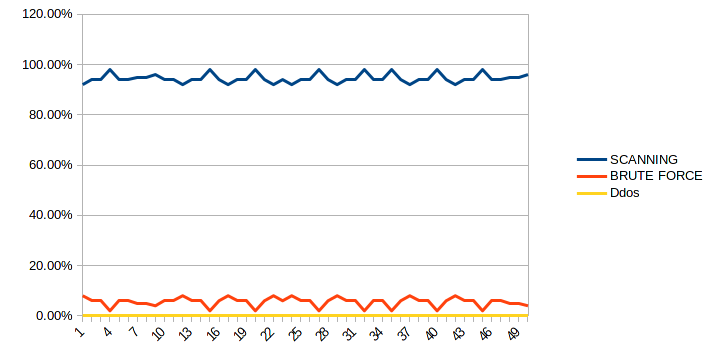
\includegraphics[scale = 0.8]{gambar/scaning}
			\caption{Grafik Deteksi Scanning}
			\label{Grafik Deteksi Scanning}
		\end{figure}
	
	
	Pada pengujian akurasi deteksi \emph{scanning} yang belum dimasukan deteksi paket normal didapatkan hasil rata rata deteksi \emph{scanning} 94.48\%, \emph{brute force} 5.52\% dan \emph{DDoS} 0\% 
	
	Berdasarkan hasil pengujian pada deteksi akurasi \emph{scanning} terdapat \emph{traffik anomali} serangan \emph{brute force} sebesar 5.52\% . Setelah menganalisa traffik \emph{scanning} dengan \emph{wireshark} didapatkan proses \emph{syn / syncronise} pada service \emph{ssh dan ftp } . Hal ini didasarkan ketika proses \emph{scanning} terjadi maka setiap \emph{service} yang aktip akan menerima proses sinkronisasi pada TCP , untuk mengetahui apakah sebuah service aktip atau tidak. 
	
		\newpage
		\noindent
		\textbf{B. Akurasi Serangan \emph{Brute Force}}
	
		Berikut akurasi serangan \emph{Brute Force} tanpa paket normal
		
\begin{table}[H]
	\centering
	\caption{Akurasi Serangan \emph{Brute Force}}
	\label{Akurasi Serangan Brute Force}
	\begin{tabular}{|c|c|c|c|c|}
		\hline
		NOMER        & SCANNING & BRUTE FORCE & DDoS   & KETERANGAN \\ \hline
		1         & 6.00\%   & 94.00\%     & 0.00\% & MEDUSA     \\ \hline
		2         & 10.00\%  & 90.00\%     & 0.00\% & HYDRA      \\ \hline
		3         & 7.00\%   & 93.00\%     & 0.00\% & MEDUSA     \\ \hline
		4         & 7.00\%   & 93.00\%     & 0.00\% & MEDUSA     \\ \hline
		5         & 7.00\%   & 93.00\%     & 0.00\% & ZERO BRUTE \\ \hline
		6         & 6.00\%   & 94.00\%     & 0.00\% & METASPLOIT \\ \hline
		7         & 6.00\%   & 94.00\%     & 0.00\% & NMAP (NSE) \\ \hline
		8         & 7.00\%   & 93.00\%     & 0.00\% & NMAP (NSE) \\ \hline
		9         & 6.00\%   & 94.00\%     & 0.00\% & HYDRA      \\ \hline
		10        & 6.89\%   & 93.11\%     & 0.00\% & MEDUSA     \\ \hline
		11        & 6.00\%   & 94.00\%     & 0.00\% & HYDRA      \\ \hline
		12        & 10.00\%  & 90.00\%     & 0.00\% & MEDUSA     \\ \hline
		13        & 7.00\%   & 93.00\%     & 0.00\% & HYDRA      \\ \hline
		14        & 7.00\%   & 93.00\%     & 0.00\% & MEDUSA     \\ \hline
		15        & 7.00\%   & 93.00\%     & 0.00\% & METASPLOIT \\ \hline
		16        & 6.00\%   & 94.00\%     & 0.00\% & NMAP (NSE) \\ \hline
		17        & 6.00\%   & 94.00\%     & 0.00\% & NMAP (NSE) \\ \hline
		18        & 7.00\%   & 93.00\%     & 0.00\% & HYDRA      \\ \hline
		19        & 6.00\%   & 94.00\%     & 0.00\% & MEDUSA     \\ \hline
		20        & 6.89\%   & 93.11\%     & 0.00\% & NMAP (NSE) \\ \hline
		21        & 7.00\%   & 93.00\%     & 0.00\% & HYDRA      \\ \hline
		22        & 6.00\%   & 94.00\%     & 0.00\% & MEDUSA     \\ \hline
		23        & 6.00\%   & 94.00\%     & 0.00\% & METASPLOIT \\ \hline
		24        & 7.00\%   & 93.00\%     & 0.00\% & MEDUSA     \\ \hline
		25        & 6.00\%   & 94.00\%     & 0.00\% & METASPLOIT \\ \hline
		
			\end{tabular}
	\end{table}

\begin{table}[H]
	\centering

	\begin{tabular}{|c|c|c|c|c|}
		\hline
		NOMER        & SCANNING & BRUTE FORCE & DDoS   & KETERANGAN \\ \hline
		26        & 6.89\%   & 93.11\%     & 0.00\% & METASPLOIT \\ \hline
		27        & 6.00\%   & 94.00\%     & 0.00\% & NMAP (NSE) \\ \hline
		28        & 10.00\%  & 90.00\%     & 0.00\% & NMAP (NSE) \\ \hline
		29        & 7.00\%   & 93.00\%     & 0.00\% & HYDRA      \\ \hline
		30        & 6.00\%   & 94.00\%     & 0.00\% & MEDUSA     \\ \hline
		31        & 7.00\%   & 93.00\%     & 0.00\% & HYDRA      \\ \hline
		32        & 6.00\%   & 94.00\%     & 0.00\% & MEDUSA     \\ \hline
		33        & 6.89\%   & 93.11\%     & 0.00\% & HYDRA      \\ \hline
		34        & 6.00\%   & 94.00\%     & 0.00\% & MEDUSA     \\ \hline
		35        & 10.00\%  & 90.00\%     & 0.00\% & METASPLOIT \\ \hline
		36        & 7.00\%   & 93.00\%     & 0.00\% & NMAP (NSE) \\ \hline
		37        & 6.00\%   & 94.00\%     & 0.00\% & NMAP (NSE) \\ \hline
		38        & 6.00\%   & 94.00\%     & 0.00\% & HYDRA      \\ \hline
		39        & 7.00\%   & 93.00\%     & 0.00\% & HYDRA      \\ \hline
		40        & 6.00\%   & 94.00\%     & 0.00\% & MEDUSA     \\ \hline
		41        & 6.89\%   & 93.11\%     & 0.00\% & METASPLOIT \\ \hline
		42        & 7.00\%   & 93.00\%     & 0.00\% & NMAP (NSE) \\ \hline
		43        & 6.00\%   & 94.00\%     & 0.00\% & NMAP (NSE) \\ \hline
		44        & 6.00\%   & 94.00\%     & 0.00\% & HYDRA      \\ \hline
		45        & 7.00\%   & 93.00\%     & 0.00\% & MEDUSA     \\ \hline
		46        & 6.00\%   & 94.00\%     & 0.00\% & NMAP (NSE) \\ \hline
		47        & 6.89\%   & 93.11\%     & 0.00\% & HYDRA      \\ \hline
		48        & 6.00\%   & 94.00\%     & 0.00\% & MEDUSA     \\ \hline
		49        & 10.00\%  & 90.00\%     & 0.00\% & METASPLOIT \\ \hline
		50        & 7.00\%   & 93.00\%     & 0.00\% & MEDUSA     \\ \hline
		RATA-RATA & 7.00\%  & 93.00\%      & 0.00\% &            \\ \hline
	\end{tabular}
\end{table}
	\begin{figure}[H]
		\centering
		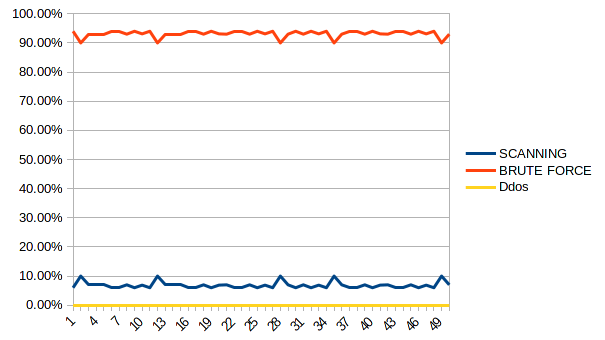
\includegraphics[scale= 0.85]{gambar/brute}
		\caption{Grafik Deteksi \emph{Brute Force} Tanpa Paket Normal}
		\label{Grafik Deteksi Brute Force Tanpa Paket Normal}
	\end{figure}
	
	
	
	Pada pengujian akurasi deteksi \emph{scanning} yang belum dimasukan deteksi paket normal didapatkan hasil rata rata deteksi \emph{scanning} 6.85\%, \emph{brute force} 93.15\% dan \emph{DDoS} 0\% 
	
	Sama halnya dengan hasil pengujian deteksi akurasi \emph{scanning} akan ditemukan \emph{anomali traffik } serangan \emph{brute force} sebesar 6.85\%. Hal ini dikarenakan ketikana akan melakukan \emph{brute force} pada service yang akan di serangan , dalam kasus ini dilakukan serangan pada \emph{service ssh}, setiap 5 detik (setingan default hydra yang digunakan untuk brute force) akan melakukan syncronisasi yang membawa payload \emph{traffik scanning} hal ini yang menyebabkan terjadinya serangan \emph{scanning} pada serangan \emph{brute force}
	
		
		
		
		\newpage
		\noindent
		\textbf{C. Akurasi Deteksi DDoS}
		
				Berikut akurasi serangan \emph{DDoS} tanpa paket normal
		
\begin{table}[H]
	\centering
	\caption{Akurasi Serangan DDoS}
	\label{Akurasi Serangan DDoS}
	\begin{tabular}{|c|c|c|c|c|}
		\hline
		NOMER        & SCANNING & BRUTE FORCE & DDoS    & KETERANGAN \\ \hline
		1         & 2.00\%   & 0.00\%      & 98.00\% & METASPLOIT \\ \hline
		2         & 3.00\%   & 0.00\%      & 97.00\% & METASPLOIT \\ \hline
		3         & 2.00\%   & 0.00\%      & 98.00\% & SLOWLORIS  \\ \hline
		4         & 2.00\%   & 0.00\%      & 98.00\% & PYLoris    \\ \hline
		5         & 3.00\%   & 0.00\%      & 97.00\% & HULK       \\ \hline
		6         & 2.00\%   & 0.00\%      & 98.00\% & HULK       \\ \hline
		7         & 2.00\%   & 0.00\%      & 98.00\% & TCP FLOOD  \\ \hline
		8         & 2.00\%   & 0.00\%      & 98.00\% & METASPLOIT \\ \hline
		9         & 2.00\%   & 0.00\%      & 98.00\% & METASPLOIT \\ \hline
		10        & 2.00\%   & 0.00\%      & 98.00\% & SLOWLORIS  \\ \hline
		11        & 2.00\%   & 0.00\%      & 98.00\% & PYLoris    \\ \hline
		12        & 3.00\%   & 0.00\%      & 97.00\% & HULK       \\ \hline
		13        & 2.00\%   & 0.00\%      & 98.00\% & HULK       \\ \hline
		14        & 2.00\%   & 0.00\%      & 98.00\% & SLOWLORIS  \\ \hline
		15        & 3.00\%   & 0.00\%      & 97.00\% & PYLoris    \\ \hline
		16        & 2.00\%   & 0.00\%      & 98.00\% & HULK       \\ \hline
		17        & 2.00\%   & 0.00\%      & 98.00\% & HULK       \\ \hline
		18        & 2.00\%   & 0.00\%      & 98.00\% & TCP FLOOD  \\ \hline
		19        & 2.00\%   & 0.00\%      & 98.00\% & TCP FLOOD  \\ \hline
		20        & 2.00\%   & 0.00\%      & 98.00\% & PYLoris    \\ \hline
		21        & 3.00\%   & 0.00\%      & 97.00\% & HULK       \\ \hline
		22        & 2.00\%   & 0.00\%      & 98.00\% & HULK       \\ \hline
		23        & 2.00\%   & 0.00\%      & 98.00\% & TCP FLOOD  \\ \hline
		24        & 3.00\%   & 0.00\%      & 97.00\% & METASPLOIT \\ \hline
		25        & 2.00\%   & 0.00\%      & 98.00\% & METASPLOIT \\ \hline
			\end{tabular}
	\end{table}
\begin{table}[H]
	\centering

	\begin{tabular}{|c|c|c|c|c|}
		\hline
		NOMER        & SCANNING & BRUTE FORCE & DDoS    & KETERANGAN \\ \hline
		26        & 3.00\%   & 0.00\%      & 97.00\% & SLOWLORIS  \\ \hline
		27        & 2.00\%   & 0.00\%      & 98.00\% & PYLoris    \\ \hline
		28        & 2.00\%   & 0.00\%      & 98.00\% & HULK       \\ \hline
		29        & 3.00\%   & 0.00\%      & 97.00\% & HULK       \\ \hline
		30        & 2.00\%   & 0.00\%      & 98.00\% & SLOWLORIS  \\ \hline
		31        & 2.00\%   & 0.00\%      & 98.00\% & PYLoris    \\ \hline
		32        & 2.00\%   & 0.00\%      & 98.00\% & HULK       \\ \hline
		33        & 2.00\%   & 0.00\%      & 98.00\% & HULK       \\ \hline
		34        & 2.00\%   & 0.00\%      & 98.00\% & HULK       \\ \hline
		35        & 2.00\%   & 0.00\%      & 98.00\% & TCP FLOOD  \\ \hline
		36        & 3.00\%   & 0.00\%      & 97.00\% & METASPLOIT \\ \hline
		37        & 2.00\%   & 0.00\%      & 98.00\% & METASPLOIT \\ \hline
		38        & 2.00\%   & 0.00\%      & 98.00\% & SLOWLORIS  \\ \hline
		39        & 3.00\%   & 0.00\%      & 97.00\% & PYLoris    \\ \hline
		40        & 2.00\%   & 0.00\%      & 98.00\% & METASPLOIT \\ \hline
		41        & 2.00\%   & 0.00\%      & 98.00\% & METASPLOIT \\ \hline
		42        & 2.00\%   & 0.00\%      & 98.00\% & SLOWLORIS  \\ \hline
		43        & 2.00\%   & 0.00\%      & 98.00\% & SLOWLORIS  \\ \hline
		44        & 2.00\%   & 0.00\%      & 98.00\% & PYLoris    \\ \hline
		45        & 3.00\%   & 0.00\%      & 97.00\% & HULK       \\ \hline
		46        & 2.00\%   & 0.00\%      & 98.00\% & HULK       \\ \hline
		47        & 2.00\%   & 0.00\%      & 98.00\% & SLOWLORIS  \\ \hline
		48        & 3.00\%   & 0.00\%      & 97.00\% & TCP FLOOD  \\ \hline
		49        & 2.00\%   & 0.00\%      & 98.00\% & METASPLOIT \\ \hline
		50        & 2.00\%   & 0.00\%      & 98.00\% & METASPLOIT \\ \hline
		RATA-RATA & 2.00\%   & 0.00\%      & 98.00\% &            \\ \hline
	\end{tabular}
\end{table}
	
	\begin{figure}[H]
		\centering
		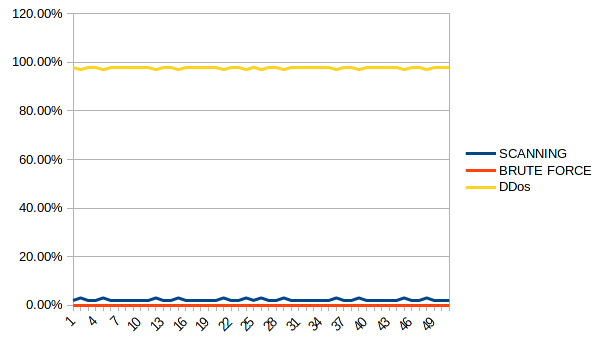
\includegraphics[scale=0.9]{gambar/DDOS}
		\caption{Grafik Deteksi DDoS Tanpa Paket Normal}
		\label{Grafik Deteksi DDoS Tanpa Paket Normal}
	\end{figure}
	
	
	Pada hasil pengujian akurasi serangan deteksi DDoS didapatkan hasil rata-rata deteksi \emph{(scanning)} 2.23\% , \emph{brute force} 0.00 \% dan \emph{DDoS} 97.73\% . 
	
	Pada serangan ini pun ditemukan \emph{traffik anomali} serangan \emph{scanning} hal ini diakibatkan karena pada saat proses  \emph{DDoS} terjadi , service yang sedang dibanjiri \emph{traffik DDoS} secara terus menurus akan melakukan proses \emph{syn/ack} kepada \emph{host} yang melakukan serangan, pada proses itu ada \emph{traffik} yang sama dengan \emph{traffik scanning} 
		
		
		\newpage
		
		\subsection{Skenario Kedua}
				
		Pada scenario ini  akan diuji masing masing akurasi deteksi serangan dengan memasukan \emph{rule} traffik normal,pengujian ini dilakukan sealama 50 kali pengujian
		serangan dimana masing-masing serangan dilakukan secara satu persatu atau terpi-
		sah disamping itu dalam penelitian tugas akhir ini dilukan monitoring penggunaan
		serangan, berikut kami sajikan table dan bagan hasil pengujian dari masing masing akurasi deteksi serangan :
		\newline
		
		
				

		\noindent
		\textbf{A. Akurasi Deteksi Scanning Dengan Memasukan Data Normal}
		
	\begin{table}[H]
		\centering
		\caption{ Akurasi Deteksi Scanning Dengan Memasukan Data Normal}
		\label{ Akurasi Deteksi Scanning Dengan Memasukan Data Normal}
		\begin{tabular}{|c|c|c|c|c|l|}
			\hline
			NOMER        & SCANNING & \begin{tabular}[c]{@{}l@{}}BRUTE \\ FORCE\end{tabular} & DDoS   & NORMAL & KETERANGAN   \\ \hline
			1         & 90.00\%  & 8.00\%      & 0.00\% & 2\%    & NMAP         \\ \hline
			2         & 91.00\%  & 6.00\%      & 0.00\% & 3\%    & NMAP         \\ \hline
			3         & 92.00\%  & 6.00\%      & 0.00\% & 2\%    & METASPLOIT   \\ \hline
			4         & 90.00\%  & 8.00\%      & 0.00\% & 2\%    & TCP SCANNING \\ \hline
			5         & 91.00\%  & 6.00\%      & 0.00\% & 3\%    & NESSUS       \\ \hline
			6         & 92.00\%  & 6.00\%      & 0.00\% & 2\%    & NESSUS       \\ \hline
			7         & 90.00\%  & 8.00\%      & 0.00\% & 2\%    & NMAP         \\ \hline
			8         & 91.00\%  & 6.00\%      & 0.00\% & 3\%    & METASPLOIT   \\ \hline
			9         & 92.00\%  & 6.00\%      & 0.00\% & 2\%    & METASPLOIT   \\ \hline
			10        & 90.00\%  & 8.00\%      & 0.00\% & 2\%    & TCP SCANNING \\ \hline
			11        & 88.00\%  & 8.00\%      & 0.00\% & 4\%    & NESSUS       \\ \hline
			12        & 90.00\%  & 6.00\%      & 0.00\% & 4\%    & TCP SCANNING \\ \hline
			13        & 91.00\%  & 6.00\%      & 0.00\% & 3\%    & METASPLOIT   \\ \hline
			14        & 92.00\%  & 6.00\%      & 0.00\% & 2\%    & METASPLOIT   \\ \hline
			15        & 90.00\%  & 8.00\%      & 0.00\% & 2\%    & TCP SCANNING \\ \hline
			16        & 88.00\%  & 8.00\%      & 0.00\% & 4\%    & NESSUS       \\ \hline
			17        & 90.00\%  & 6.00\%      & 0.00\% & 4\%    & NESSUS       \\ \hline
			18        & 88.00\%  & 8.00\%      & 0.00\% & 4\%    & NMAP         \\ \hline
			19        & 90.00\%  & 6.00\%      & 0.00\% & 4\%    & METASPLOIT   \\ \hline
				\end{tabular}
		\end{table}
	
		\begin{table}[H]
		\centering

		\begin{tabular}{|c|c|c|c|c|l|}
			\hline
			NOMER        & SCANNING & \begin{tabular}[c]{@{}l@{}}BRUTE \\ FORCE\end{tabular} & DDoS   & NORMAL & KETERANGAN   \\ \hline
	
			
			20        & 91.00\%  & 6.00\%      & 0.00\% & 3\%    & METASPLOIT   \\ \hline
			21        & 92.00\%  & 6.00\%      & 0.00\% & 2\%    & TCP SCANNING \\ \hline
			22        & 90.00\%  & 8.00\%      & 0.00\% & 2\%    & NESSUS       \\ \hline
			23        & 88.00\%  & 8.00\%      & 0.00\% & 4\%    & TCP SCANNING \\ \hline
			24        & 90.00\%  & 6.00\%      & 0.00\% & 4\%    & METASPLOIT   \\ \hline
			25        & 90.00\%  & 8.00\%      & 0.00\% & 2\%    & NESSUS       \\ \hline
			26        & 88.00\%  & 8.00\%      & 0.00\% & 4\%    & TCP SCANNING \\ \hline
			27        & 90.00\%  & 6.00\%      & 0.00\% & 4\%    & METASPLOIT   \\ \hline
			28        & 88.00\%  & 8.00\%      & 0.00\% & 4\%    & METASPLOIT   \\ \hline
			29        & 90.00\%  & 6.00\%      & 0.00\% & 4\%    & TCP SCANNING \\ \hline
			30        & 91.00\%  & 6.00\%      & 0.00\% & 3\%    & NESSUS       \\ \hline
			31        & 92.00\%  & 6.00\%      & 0.00\% & 2\%    & NESSUS       \\ \hline
			32        & 90.00\%  & 8.00\%      & 0.00\% & 2\%    & NMAP         \\ \hline
			33        & 90.00\%  & 6.00\%      & 0.00\% & 4\%    & METASPLOIT   \\ \hline
			34        & 91.00\%  & 6.00\%      & 0.00\% & 3\%    & METASPLOIT   \\ \hline
			35        & 92.00\%  & 6.00\%      & 0.00\% & 2\%    & TCP SCANNING \\ \hline
			36        & 90.00\%  & 8.00\%      & 0.00\% & 2\%    & NESSUS       \\ \hline
			37        & 88.00\%  & 8.00\%      & 0.00\% & 4\%    & TCP SCANNING \\ \hline
			38        & 90.00\%  & 6.00\%      & 0.00\% & 4\%    & METASPLOIT   \\ \hline
			39        & 90.00\%  & 8.00\%      & 0.00\% & 2\%    & METASPLOIT   \\ \hline
			40        & 88.00\%  & 8.00\%      & 0.00\% & 4\%    & TCP SCANNING \\ \hline
			41        & 90.00\%  & 6.00\%      & 0.00\% & 4\%    & NESSUS       \\ \hline
			42        & 90.00\%  & 6.00\%      & 0.00\% & 4\%    & NESSUS       \\ \hline
			43        & 91.00\%  & 6.00\%      & 0.00\% & 3\%    & NMAP         \\ \hline
			44        & 92.00\%  & 6.00\%      & 0.00\% & 2\%    & METASPLOIT   \\ \hline
			45        & 90.00\%  & 8.00\%      & 0.00\% & 2\%    & METASPLOIT   \\ \hline
			46        & 88.00\%  & 8.00\%      & 0.00\% & 4\%    & TCP SCANNING \\ \hline
			47        & 90.00\%  & 6.00\%      & 0.00\% & 4\%    & NESSUS       \\ \hline
			48        & 90.00\%  & 8.00\%      & 0.00\% & 2\%    & TCP SCANNING \\ \hline
			49        & 88.00\%  & 8.00\%      & 0.00\% & 4\%    & METASPLOIT   \\ \hline
			50        & 90.00\%  & 6.00\%      & 0.00\% & 4\%    & NMAP         \\ \hline
			RATA-RATA & 90.08\%  & 6.88\%      & 0.00\% & 3.04\% &              \\ \hline
		\end{tabular}
	\end{table}
	
	
	
	\begin{figure}[H]
		\centering
		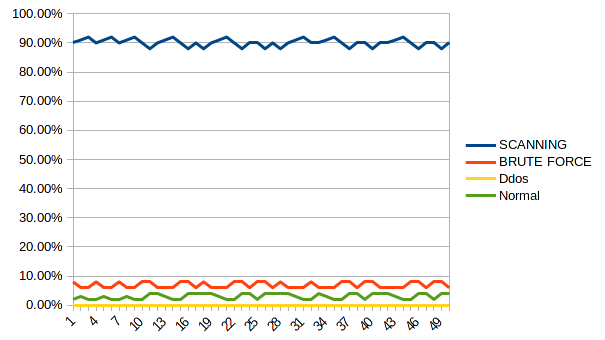
\includegraphics[scale=0.9]{gambar/ddosnormal}
		\caption{Grafik Deteksi Scanning  Dengan Paket Normal}
		\label{Grafik Deteksi Scanning  Dengan Paket Normal}
	\end{figure}
	
	
	Pada pengujian yang ini didapatkan hasil akurasi \emph{scanning} 90.08\% \emph{brute force} 6.88\% \emph{DDoS} 0.0\% dan paket normal 3.04 \%.
		
	Sama halnya dengan peengujian sebelumnya akan terdeteksi juga serangan \emph{brute force}
	
	Setalah memasukan deteksi \emph{traffik} normal akan didapatkan pada serangan \emph{scanning} sebesar 3.04\% hal itu diakibatkan kerana proses \emph{echo-reply} paket \emph{icmp}
	

		\newpage
		\noindent
		\textbf{B. Akurasi Deteksi Brute Force Dengan Memasukan Data Normal}
		
\begin{table}[H]
	\centering
	\caption{Akurasi Deteksi Brute Force Dengan Memasukan Data Normal}
	\label{Akurasi Deteksi Brute Force Dengan Memasukan Data Normal}
	\begin{tabular}{|c|c|c|c|c|l|}
		\hline
		NOMER        & SCANNING & \begin{tabular}[c]{@{}l@{}}BRUTE \\ FORCE\end{tabular} & DDoS   & NORMAL & KETERANGAN   \\ \hline
		1         & 6.00\%   & 88.00\%     & 0.00\% & 6\%    & MEDUSA     \\ \hline
		2         & 6.00\%   & 87.00\%     & 0.00\% & 7\%    & HYDRA      \\ \hline
		3         & 7.00\%   & 88.00\%     & 0.00\% & 5\%    & MEDUSA     \\ \hline
		4         & 7.00\%   & 87.00\%     & 0.00\% & 6\%    & MEDUSA     \\ \hline
		5         & 7.00\%   & 87.00\%     & 0.00\% & 6\%    & ZERO BRUTE \\ \hline
		6         & 6.00\%   & 86.00\%     & 0.00\% & 8\%    & METASPLOIT \\ \hline
		7         & 6.00\%   & 88.00\%     & 0.00\% & 6\%    & NMAP (NSE) \\ \hline
		8         & 6.00\%   & 87.00\%     & 0.00\% & 7\%    & NMAP (NSE) \\ \hline
		9         & 7.00\%   & 88.00\%     & 0.00\% & 5\%    & HYDRA      \\ \hline
		10        & 7.00\%   & 87.00\%     & 0.00\% & 6\%    & MEDUSA     \\ \hline
		11        & 7.00\%   & 87.00\%     & 0.00\% & 6\%    & HYDRA      \\ \hline
		12        & 6.00\%   & 86.00\%     & 0.00\% & 8\%    & MEDUSA     \\ \hline
		13        & 7.00\%   & 87.00\%     & 0.00\% & 6\%    & HYDRA      \\ \hline
		14        & 7.00\%   & 87.00\%     & 0.00\% & 6\%    & MEDUSA     \\ \hline
		15        & 6.00\%   & 86.00\%     & 0.00\% & 8\%    & METASPLOIT \\ \hline
		16        & 6.00\%   & 88.00\%     & 0.00\% & 6\%    & NMAP (NSE) \\ \hline
		17        & 6.00\%   & 87.00\%     & 0.00\% & 7\%    & NMAP (NSE) \\ \hline
		18        & 7.00\%   & 88.00\%     & 0.00\% & 5\%    & HYDRA      \\ \hline
		19        & 7.00\%   & 87.00\%     & 0.00\% & 6\%    & MEDUSA     \\ \hline
		20        & 6.00\%   & 88.00\%     & 0.00\% & 6\%    & NMAP (NSE) \\ \hline
		21        & 6.00\%   & 87.00\%     & 0.00\% & 7\%    & HYDRA      \\ \hline
		22        & 7.00\%   & 88.00\%     & 0.00\% & 5\%    & MEDUSA     \\ \hline
		23        & 7.00\%   & 87.00\%     & 0.00\% & 6\%    & METASPLOIT \\ \hline
		24        & 7.00\%   & 87.00\%     & 0.00\% & 6\%    & MEDUSA     \\ \hline
		25        & 6.00\%   & 86.00\%     & 0.00\% & 8\%    & METASPLOIT \\ \hline
	\end{tabular}
\end{table}
		
\begin{table}[H]
	\centering

	\begin{tabular}{|c|c|c|c|c|l|}
		\hline
		NOMER        & SCANNING & \begin{tabular}[c]{@{}l@{}}BRUTE \\ FORCE\end{tabular} & DDoS   & NORMAL & KETERANGAN   \\ \hline
		26        & 6.00\%   & 88.00\%     & 0.00\% & 6\%    & METASPLOIT \\ \hline
		27        & 6.00\%   & 87.00\%     & 0.00\% & 7\%    & NMAP (NSE) \\ \hline
		28        & 7.00\%   & 88.00\%     & 0.00\% & 5\%    & NMAP (NSE) \\ \hline
		29        & 7.00\%   & 87.00\%     & 0.00\% & 6\%    & HYDRA      \\ \hline
		30        & 7.00\%   & 87.00\%     & 0.00\% & 6\%    & MEDUSA     \\ \hline
		31        & 6.00\%   & 86.00\%     & 0.00\% & 8\%    & HYDRA      \\ \hline
		32        & 7.00\%   & 87.00\%     & 0.00\% & 6\%    & MEDUSA     \\ \hline
		33        & 7.00\%   & 87.00\%     & 0.00\% & 6\%    & HYDRA      \\ \hline
		34        & 6.00\%   & 86.00\%     & 0.00\% & 8\%    & MEDUSA     \\ \hline
		35        & 6.00\%   & 88.00\%     & 0.00\% & 6\%    & METASPLOIT \\ \hline
		36        & 6.00\%   & 87.00\%     & 0.00\% & 7\%    & NMAP (NSE) \\ \hline
		37        & 7.00\%   & 88.00\%     & 0.00\% & 5\%    & NMAP (NSE) \\ \hline
		38        & 7.00\%   & 87.00\%     & 0.00\% & 6\%    & HYDRA      \\ \hline
		39        & 7.00\%   & 87.00\%     & 0.00\% & 6\%    & HYDRA      \\ \hline
		40        & 6.00\%   & 86.00\%     & 0.00\% & 8\%    & MEDUSA     \\ \hline
		41        & 7.00\%   & 87.00\%     & 0.00\% & 6\%    & METASPLOIT \\ \hline
		42        & 7.00\%   & 87.00\%     & 0.00\% & 6\%    & NMAP (NSE) \\ \hline
		43        & 6.00\%   & 86.00\%     & 0.00\% & 8\%    & NMAP (NSE) \\ \hline
		44        & 6.00\%   & 88.00\%     & 0.00\% & 6\%    & HYDRA      \\ \hline
		45        & 6.00\%   & 87.00\%     & 0.00\% & 7\%    & MEDUSA     \\ \hline
		46        & 7.00\%   & 88.00\%     & 0.00\% & 5\%    & NMAP (NSE) \\ \hline
		47        & 7.00\%   & 87.00\%     & 0.00\% & 6\%    & HYDRA      \\ \hline
		48        & 6.00\%   & 88.00\%     & 0.00\% & 6\%    & MEDUSA     \\ \hline
		49        & 6.00\%   & 87.00\%     & 0.00\% & 7\%    & METASPLOIT \\ \hline
		50        & 7.00\%   & 88.00\%     & 0.00\% & 5\%    & MEDUSA     \\ \hline
		RATA-RATA & 6.52\%   & 87.15\%     & 0.00\% & 6.33\% &            \\ \hline
	\end{tabular}
\end{table}


\begin{figure}[H]
	\centering
	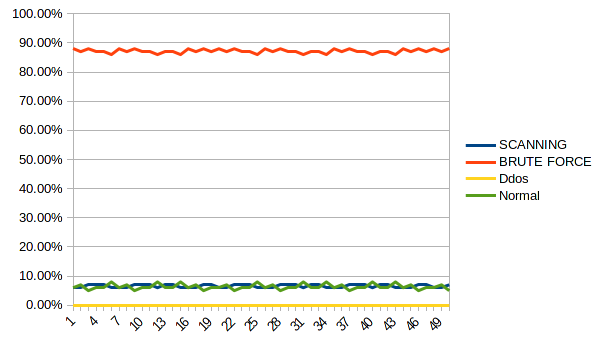
\includegraphics[scale=0.9]{gambar/brutenormal}
	\caption{Grafik Deteksi Brute Force Dengan Paket Normal}
	\label{Grafik Deteksi Brute Force Dengan  Paket Normal}
\end{figure}

	
Pada pengujian yang ini didapatkan hasil akurasi \emph{scanning} 6.52\% \emph{brute force} 87.16\% \emph{DDoS} 0.0\% dan paket normal 6.32 \%.

Sama halnya dengan peengujian sebelumnya akan terdeteksi juga serangan \emph{scanning}

Setalah memasukan deteksi \emph{traffik} normal akan didapatkan pada serangan \emph{scanning} sebesar 6.32\% hal itu diakibatkan kerana proses \emph{echo-reply} paket \emph{icmp}



		\newpage
		\noindent
		\textbf{C. Akurasi Deteksi DDoS Dengan Memasukan Data Normal}
\begin{table}[H]
	\centering
	\caption{Akurasi Deteksi DDoS Dengan Memasukan Data Normal}
	\label{Akurasi Deteksi DDoS Dengan Memasukan Data Normal}
	\begin{tabular}{|c|c|c|c|c|l|}
		\hline
		NOMER        & SCANNING & \begin{tabular}[c]{@{}c@{}}BRUTE \\ FORCE\end{tabular} & DDoS    & NORMAL & KETERANGAN \\ \hline
		1         & 2.00\%   & 0.00\%                                                 & 98.00\% & 0\%    & METASPLOIT \\ \hline
		2         & 3.00\%   & 0.00\%                                                 & 97.00\% & 0\%    & METASPLOIT \\ \hline
		3         & 2.00\%   & 0.00\%                                                 & 96.00\% & 2\%    & SLOWLORIS  \\ \hline
		4         & 2.00\%   & 0.00\%                                                 & 98.00\% & 0\%    & PYLoris    \\ \hline
		5         & 3.00\%   & 0.00\%                                                 & 96.00\% & 1\%    & HULK       \\ \hline
		6         & 2.00\%   & 0.00\%                                                 & 98.00\% & 0\%    & HULK       \\ \hline
		7         & 2.00\%   & 0.00\%                                                 & 98.00\% & 0\%    & TCP FLOOD  \\ \hline
		8         & 2.00\%   & 0.00\%                                                 & 98.00\% & 0\%    & METASPLOIT \\ \hline
		9         & 2.00\%   & 0.00\%                                                 & 98.00\% & 0\%    & METASPLOIT \\ \hline
		10        & 2.00\%   & 0.00\%                                                 & 98.00\% & 0\%    & SLOWLORIS  \\ \hline
		11        & 2.00\%   & 0.00\%                                                 & 98.00\% & 0\%    & PYLoris    \\ \hline
		12        & 3.00\%   & 0.00\%                                                 & 97.00\% & 0\%    & HULK       \\ \hline
		13        & 2.00\%   & 0.00\%                                                 & 98.00\% & 0\%    & HULK       \\ \hline
		14        & 2.00\%   & 0.00\%                                                 & 98.00\% & 0\%    & SLOWLORIS  \\ \hline
		15        & 3.00\%   & 0.00\%                                                 & 97.00\% & 0\%    & PYLoris    \\ \hline
		16        & 2.00\%   & 0.00\%                                                 & 96.00\% & 2\%    & HULK       \\ \hline
		17        & 2.00\%   & 0.00\%                                                 & 98.00\% & 0\%    & HULK       \\ \hline
		18        & 3.00\%   & 0.00\%                                                 & 96.00\% & 1\%    & TCP FLOOD  \\ \hline
		19        & 2.00\%   & 0.00\%                                                 & 98.00\% & 0\%    & TCP FLOOD  \\ \hline
		20        & 2.00\%   & 0.00\%                                                 & 98.00\% & 0\%    & PYLoris    \\ \hline
		21        & 2.00\%   & 0.00\%                                                 & 98.00\% & 0\%    & HULK       \\ \hline
		22        & 2.00\%   & 0.00\%                                                 & 98.00\% & 0\%    & HULK       \\ \hline
		23        & 2.00\%   & 0.00\%                                                 & 98.00\% & 0\%    & TCP FLOOD  \\ \hline
		24        & 2.00\%   & 0.00\%                                                 & 98.00\% & 0\%    & METASPLOIT \\ \hline
		
	\end{tabular}
\end{table}
		
\begin{table}[H]
	\centering
	\begin{tabular}{|c|c|c|c|c|l|}
		\hline
		NO        & SCANNING & \begin{tabular}[c]{@{}c@{}}BRUTE \\ FORCE\end{tabular} & DDoS    & NORMAL & KETERANGAN \\ \hline
		
		25        & 3.00\%   & 0.00\%                                                 & 97.00\% & 0\%    & METASPLOIT \\ \hline
		26        & 2.00\%   & 0.00\%                                                 & 98.00\% & 0\%    & SLOWLORIS  \\ \hline
		27        & 2.00\%   & 0.00\%                                                 & 98.00\% & 0\%    & PYLoris    \\ \hline
		28        & 3.00\%   & 0.00\%                                                 & 97.00\% & 0\%    & HULK       \\ \hline
		29        & 2.00\%   & 0.00\%                                                 & 96.00\% & 2\%    & HULK       \\ \hline
		30        & 2.00\%   & 0.00\%                                                 & 98.00\% & 0\%    & SLOWLORIS  \\ \hline
		31        & 3.00\%   & 0.00\%                                                 & 96.00\% & 1\%    & PYLoris    \\ \hline
		32        & 2.00\%   & 0.00\%                                                 & 98.00\% & 0\%    & HULK       \\ \hline
		33        & 2.00\%   & 0.00\%                                                 & 98.00\% & 0\%    & HULK       \\ \hline
		34        & 2.00\%   & 0.00\%                                                 & 98.00\% & 0\%    & HULK       \\ \hline
		35        & 3.00\%   & 0.00\%                                                 & 96.00\% & 1\%    & TCP FLOOD  \\ \hline
		36        & 2.00\%   & 0.00\%                                                 & 98.00\% & 0\%    & METASPLOIT \\ \hline
		37        & 2.00\%   & 0.00\%                                                 & 98.00\% & 0\%    & METASPLOIT \\ \hline
		38        & 2.00\%   & 0.00\%                                                 & 98.00\% & 0\%    & SLOWLORIS  \\ \hline
		39        & 2.00\%   & 0.00\%                                                 & 98.00\% & 0\%    & PYLoris    \\ \hline
		40        & 2.00\%   & 0.00\%                                                 & 98.00\% & 0\%    & METASPLOIT \\ \hline
		41        & 2.00\%   & 0.00\%                                                 & 98.00\% & 0\%    & METASPLOIT \\ \hline
		42        & 3.00\%   & 0.00\%                                                 & 97.00\% & 0\%    & SLOWLORIS  \\ \hline
		43        & 2.00\%   & 0.00\%                                                 & 98.00\% & 0\%    & SLOWLORIS  \\ \hline
		44        & 2.00\%   & 0.00\%                                                 & 98.00\% & 0\%    & PYLoris    \\ \hline
		45        & 3.00\%   & 0.00\%                                                 & 97.00\% & 0\%    & HULK       \\ \hline
		46        & 2.00\%   & 0.00\%                                                 & 96.00\% & 2\%    & HULK       \\ \hline
		47        & 2.00\%   & 0.00\%                                                 & 98.00\% & 0\%    & SLOWLORIS  \\ \hline
		48        & 3.00\%   & 0.00\%                                                 & 97.00\% & 0\%    & TCP FLOOD  \\ \hline
		49        & 2.00\%   & 0.00\%                                                 & 98.00\% & 0\%    & METASPLOIT \\ \hline
		50        & 2.00\%   & 0.00\%                                                 & 98.00\% & 0\%    & METASPLOIT \\ \hline
		RATA-RATA & 3.00\%   & 0.00\%                                                 & 97.00\% & 0\%    &            \\ \hline
	\end{tabular}
\end{table}





	\begin{figure}[H]
		\centering
		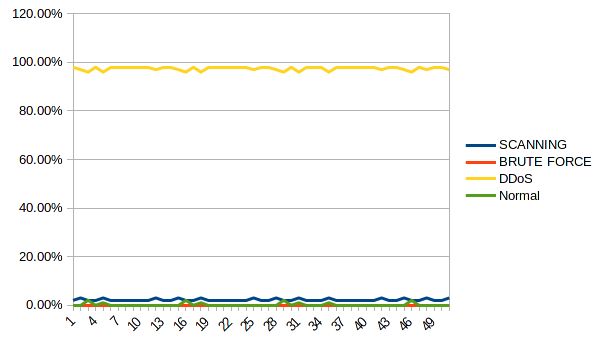
\includegraphics[scale=0.9]{gambar/ddosnormal1}
		\caption{Grafik Deteksi DDoS Dengan Paket Normal}
		\label{Grafik DDos Force Dengan  Paket Normal}
	\end{figure}
	
	
	
	Pada pengujian yang ini didapatkan hasil akurasi \emph{scanning} 2.25\% \emph{brute force} 0.00\% \emph{DDoS} 97.51\% dan paket normal 0.24 \%.
	
	Sama halnya dengan peengujian sebelumnya akan terdeteksi juga serangan \emph{scanning}
	
	Setalah memasukan deteksi \emph{traffik} normal akan didapatkan pada serangan \emph{scanning} sebesar 0.24\% hal itu diakibatkan kerana proses \emph{echo-reply} paket \emph{icmp}
	
	
	
	\newpage
	\subsection{Skenario Ketiga}
	Pada pengujian di skenario ini , akan ditunjukan perbandingan akurasi deteksi antara menggunakan paket normal dan tidak menggunakan paket normal 
	
	\noindent
	\textbf{A. Perbandingan Akurasi Deteksi Scanning }
	
	\begin{table}[H]
		\centering
		\caption{ Perbandingan Akurasi Deteksi Scanning}
		\label{Perbandingan Akurasi Deteksi Scanning}
		\begin{tabular}{|l|l|l|l|l|l|}
			\hline
no & \multicolumn{1}{c|}{\begin{tabular}[c]{@{}c@{}}Scanning tanpa\\ paket normal\end{tabular}} & \multicolumn{1}{c|}{\begin{tabular}[c]{@{}c@{}}Scanning dengan \\ paket normal\end{tabular}} & no & \multicolumn{1}{c|}{\begin{tabular}[c]{@{}c@{}}Scanning tanpa \\ paket normal\end{tabular}} & \multicolumn{1}{c|}{\begin{tabular}[c]{@{}c@{}}Scanning dengan \\ paket normal\end{tabular}} \\ \hline

			1  & 92.00\%                                                               & 90.00\%                                                                 & 26 & 94.00\%                                                                & 88.00\%                                                                 \\ \hline
			2  & 94.00\%                                                               & 91.00\%                                                                 & 27 & 98.00\%                                                                & 90.00\%                                                                 \\ \hline
			3  & 94.00\%                                                               & 92.00\%                                                                 & 28 & 94.00\%                                                                & 88.00\%                                                                 \\ \hline
			4  & 98.00\%                                                               & 90.00\%                                                                 & 29 & 92.00\%                                                                & 90.00\%                                                                 \\ \hline
			5  & 94.00\%                                                               & 91.00\%                                                                 & 30 & 94.00\%                                                                & 91.00\%                                                                 \\ \hline
			6  & 94.00\%                                                               & 92.00\%                                                                 & 31 & 94.00\%                                                                & 92.00\%                                                                 \\ \hline
			7  & 95.00\%                                                               & 90.00\%                                                                 & 32 & 98.00\%                                                                & 90.00\%                                                                 \\ \hline
			8  & 95.00\%                                                               & 91.00\%                                                                 & 33 & 94.00\%                                                                & 90.00\%                                                                 \\ \hline
			9  & 96.00\%                                                               & 92.00\%                                                                 & 34 & 94.00\%                                                                & 91.00\%                                                                 \\ \hline
			10 & 94.00\%                                                               & 90.00\%                                                                 & 35 & 98.00\%                                                                & 92.00\%                                                                 \\ \hline
			11 & 94.00\%                                                               & 88.00\%                                                                 & 36 & 94.00\%                                                                & 90.00\%                                                                 \\ \hline
			12 & 92.00\%                                                               & 90.00\%                                                                 & 37 & 92.00\%                                                                & 88.00\%                                                                 \\ \hline
			13 & 94.00\%                                                               & 91.00\%                                                                 & 38 & 94.00\%                                                                & 90.00\%                                                                 \\ \hline
			14 & 94.00\%                                                               & 92.00\%                                                                 & 39 & 94.00\%                                                                & 90.00\%                                                                 \\ \hline
			15 & 98.00\%                                                               & 90.00\%                                                                 & 40 & 98.00\%                                                                & 88.00\%                                                                 \\ \hline
			16 & 94.00\%                                                               & 88.00\%                                                                 & 41 & 94.00\%                                                                & 90.00\%                                                                 \\ \hline
			17 & 92.00\%                                                               & 90.00\%                                                                 & 42 & 92.00\%                                                                & 90.00\%                                                                 \\ \hline
			18 & 94.00\%                                                               & 88.00\%                                                                 & 43 & 94.00\%                                                                & 91.00\%                                                                 \\ \hline
			19 & 94.00\%                                                               & 90.00\%                                                                 & 44 & 94.00\%                                                                & 92.00\%                                                                 \\ \hline
			20 & 98.00\%                                                               & 91.00\%                                                                 & 45 & 98.00\%                                                                & 90.00\%                                                                 \\ \hline
			21 & 94.00\%                                                               & 92.00\%                                                                 & 46 & 94.00\%                                                                & 88.00\%                                                                 \\ \hline
			22 & 92.00\%                                                               & 90.00\%                                                                 & 47 & 94.00\%                                                                & 90.00\%                                                                 \\ \hline
			23 & 94.00\%                                                               & 88.00\%                                                                 & 48 & 95.00\%                                                                & 90.00\%                                                                 \\ \hline
			24 & 92.00\%                                                               & 90.00\%                                                                 & 49 & 95.00\%                                                                & 88.00\%                                                                 \\ \hline
			25 & 94.00\%                                                               & 90.00\%                                                                 & 50 & 96.00\%                                                                & 90.00\%                                                                 \\ \hline
			&                                                                       & \multicolumn{2}{l|}{rata - rata}                                             & 94.48\%                                                                & 90.08\%                                                                 \\ \hline
		\end{tabular}
	\end{table}

\begin{figure}[H]
	\centering
	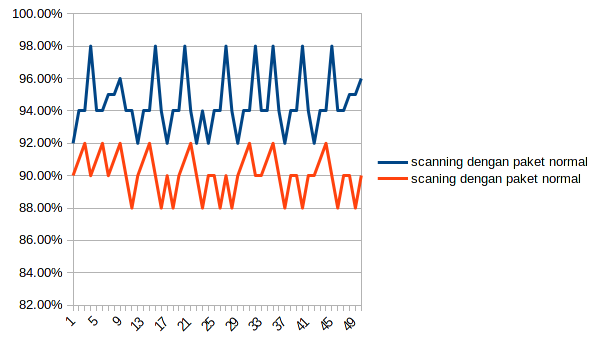
\includegraphics[scale=0.8]{gambar/pscanning}
	\caption{Perbandinan Akurasi Deteksi Scanning}
	\label{Perbandinan Akurasi Deteksi Scanning}
\end{figure}

Pada hasil perbandingan ini didapatkan hasil \emph{(scanning)} tanpa paket normal 94.48\% dan dengan paket normal 90.08\%. Seperti hasil penelitian pada skenario kedua hasil yang didapatkan pada hasil \emph{scanning} tanpa paket normal lebih besar dengan \emph{scanning} yang menggunakan paket normal . Hal ini diakibatkan karena serangan \emph{scanning} memerlukan echo-replay terhadap target

\newpage
\noindent
\textbf{B. Perbandingan Akurasi Deteksi Brute Force }

\begin{table}[H]
	\centering
	\caption{Perbandingan Akurasi Deteksi Brute Force}
	\label{Perbandingan Akurasi Deteksi Brute Force}
	\begin{tabular}{|l|l|l|l|l|l|}
		\hline
		no & \multicolumn{1}{c|}{\begin{tabular}[c]{@{}c@{}}Brute force tanpa\\ paket normal\end{tabular}} & \multicolumn{1}{c|}{\begin{tabular}[c]{@{}c@{}}Brute force dengan \\ paket normal\end{tabular}} & no & \multicolumn{1}{c|}{\begin{tabular}[c]{@{}c@{}}Brute forcetanpa \\ paket normal\end{tabular}} & \multicolumn{1}{c|}{\begin{tabular}[c]{@{}c@{}}Brute force dengan\\  paket normal\end{tabular}} \\ \hline
		1  & 94.00\%                                                                                       & 88.00\%                                                                                         & 26 & 93.11\%                                                                                       & 88.00\%                                                                                         \\ \hline
		2  & 90.00\%                                                                                       & 87.00\%                                                                                         & 27 & 94.00\%                                                                                       & 87.00\%                                                                                         \\ \hline
		3  & 93.00\%                                                                                       & 88.00\%                                                                                         & 28 & 90.00\%                                                                                       & 88.00\%                                                                                         \\ \hline
		4  & 93.00\%                                                                                       & 87.00\%                                                                                         & 29 & 93.00\%                                                                                       & 87.00\%                                                                                         \\ \hline
		5  & 93.00\%                                                                                       & 87.00\%                                                                                         & 30 & 94.00\%                                                                                       & 87.00\%                                                                                         \\ \hline
		6  & 94.00\%                                                                                       & 86.00\%                                                                                         & 31 & 93.00\%                                                                                       & 86.00\%                                                                                         \\ \hline
		7  & 94.00\%                                                                                       & 88.00\%                                                                                         & 32 & 94.00\%                                                                                       & 87.00\%                                                                                         \\ \hline
		8  & 93.00\%                                                                                       & 87.00\%                                                                                         & 33 & 93.11\%                                                                                       & 87.00\%                                                                                         \\ \hline
		9  & 94.00\%                                                                                       & 88.00\%                                                                                         & 34 & 94.00\%                                                                                       & 86.00\%                                                                                         \\ \hline
		10 & 93.11\%                                                                                       & 87.00\%                                                                                         & 35 & 90.00\%                                                                                       & 88.00\%                                                                                         \\ \hline
		11 & 94.00\%                                                                                       & 87.00\%                                                                                         & 36 & 93.00\%                                                                                       & 87.00\%                                                                                         \\ \hline
		12 & 90.00\%                                                                                       & 86.00\%                                                                                         & 37 & 94.00\%                                                                                       & 88.00\%                                                                                         \\ \hline
		13 & 93.00\%                                                                                       & 87.00\%                                                                                         & 38 & 94.00\%                                                                                       & 87.00\%                                                                                         \\ \hline
		14 & 93.00\%                                                                                       & 87.00\%                                                                                         & 39 & 93.00\%                                                                                       & 87.00\%                                                                                         \\ \hline
		15 & 93.00\%                                                                                       & 86.00\%                                                                                         & 40 & 94.00\%                                                                                       & 86.00\%                                                                                         \\ \hline
		16 & 94.00\%                                                                                       & 88.00\%                                                                                         & 41 & 93.11\%                                                                                       & 87.00\%                                                                                         \\ \hline
		17 & 94.00\%                                                                                       & 87.00\%                                                                                         & 42 & 93.00\%                                                                                       & 87.00\%                                                                                         \\ \hline
		18 & 93.00\%                                                                                       & 88.00\%                                                                                         & 43 & 94.00\%                                                                                       & 86.00\%                                                                                         \\ \hline
		19 & 94.00\%                                                                                       & 87.00\%                                                                                         & 44 & 94.00\%                                                                                       & 88.00\%                                                                                         \\ \hline
		20 & 93.11\%                                                                                       & 88.00\%                                                                                         & 45 & 93.00\%                                                                                       & 87.00\%                                                                                         \\ \hline
		21 & 93.00\%                                                                                       & 87.00\%                                                                                         & 46 & 94.00\%                                                                                       & 88.00\%                                                                                         \\ \hline
		22 & 94.00\%                                                                                       & 88.00\%                                                                                         & 47 & 93.11\%                                                                                       & 87.00\%                                                                                         \\ \hline
		23 & 94.00\%                                                                                       & 87.00\%                                                                                         & 48 & 94.00\%                                                                                       & 88.00\%                                                                                         \\ \hline
		24 & 93.00\%                                                                                       & 87.00\%                                                                                         & 49 & 90.00\%                                                                                       & 87.00\%                                                                                         \\ \hline
		25 & 94.00\%                                                                                       & 86.00\%                                                                                         & 50 & 93.00\%                                                                                       & 88.00\%                                                                                         \\ \hline
		&                                                                                               & \multicolumn{2}{l|}{rata - rata}                                                                     & 93.15\%                                                                                       & 87.16\%                                                                                         \\ \hline
	\end{tabular}
\end{table}



\begin{figure}[H]
	\centering
	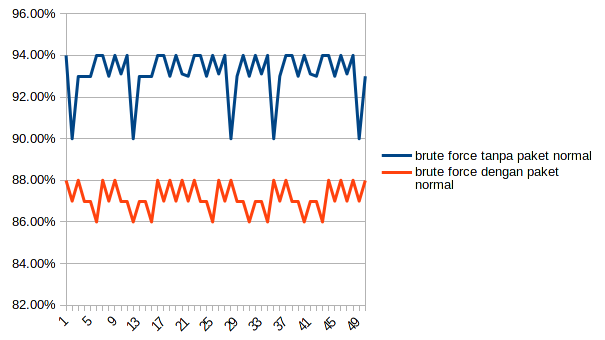
\includegraphics[scale=0.9]{gambar/pbrute}
	\caption{Perbandingan Akurasi Deteksi Brute Force}
	\label{Perbandingan Akurasi Deteksi Brute Force}
\end{figure}

Pada hasil perbandingan ini didapatkan hasil \emph{(brute force)} tanpa paket normal 93.15\% dan dengan paket normal 87.16\%. Seperti hasil penelitian pada skenario kedua hasil yang didapatkan pada hasil \emph{brute force} tanpa paket normal lebih besar dengan \emph{brute force} yang menggunakan paket normal . Hal ini diakibatkan karena serangan \emph{brute force} memerlukan echo-replay terhadap target hal ini juga didapatkan pada serangan \emph{scanning}

	\newpage
	\noindent
	\textbf{C. Perbandingan Akurasi Deteksi DDoS }
	
	
	
	\begin{table}[H]
		\centering
		\caption{ Perbandinan Akurasi Deteksi DDoS}
		\label{ Perbandinan Akurasi Deteksi DDoS}
		\begin{tabular}{|l|l|l|l|l|l|}
			\hline
no & \multicolumn{1}{c|}{\begin{tabular}[c]{@{}c@{}}DDoS tanpa\\ paket normal\end{tabular}} & \multicolumn{1}{c|}{\begin{tabular}[c]{@{}c@{}}DDoS dengan \\ paket normal\end{tabular}} & no & \multicolumn{1}{c|}{\begin{tabular}[c]{@{}c@{}}DDoS tanpa \\ paket normal\end{tabular}} & \multicolumn{1}{c|}{\begin{tabular}[c]{@{}c@{}}DDoS dengan \\ paket normal\end{tabular}} \\ \hline
			1  & 98.00\%                 & 98.00\%                    & 26  & 97.00\%                 & 98.00\%                  \\ \hline
			2  & 97.00\%                 & 97.00\%                    & 27  & 98.00\%                 & 98.00\%                  \\ \hline
			3  & 98.00\%                 & 96.00\%                    & 28  & 98.00\%                 & 97.00\%                  \\ \hline
			4  & 98.00\%                 & 98.00\%                    & 29  & 97.00\%                 & 96.00\%                  \\ \hline
			5  & 97.00\%                 & 96.00\%                    & 30  & 98.00\%                 & 98.00\%                  \\ \hline
			6  & 98.00\%                 & 98.00\%                    & 31  & 98.00\%                 & 96.00\%                  \\ \hline
			7  & 98.00\%                 & 98.00\%                    & 32  & 98.00\%                 & 98.00\%                  \\ \hline
			8  & 98.00\%                 & 98.00\%                    & 33  & 98.00\%                 & 98.00\%                  \\ \hline
			9  & 98.00\%                 & 98.00\%                    & 34  & 98.00\%                 & 98.00\%                  \\ \hline
			10 & 98.00\%                 & 98.00\%                    & 35  & 98.00\%                 & 96.00\%                  \\ \hline
			11 & 98.00\%                 & 98.00\%                    & 36  & 97.00\%                 & 98.00\%                  \\ \hline
			12 & 97.00\%                 & 97.00\%                    & 37  & 98.00\%                 & 98.00\%                  \\ \hline
			13 & 98.00\%                 & 98.00\%                    & 38  & 98.00\%                 & 98.00\%                  \\ \hline
			14 & 98.00\%                 & 98.00\%                    & 39  & 97.00\%                 & 98.00\%                  \\ \hline
			15 & 97.00\%                 & 97.00\%                    & 40  & 98.00\%                 & 98.00\%                  \\ \hline
			16 & 98.00\%                 & 96.00\%                    & 41  & 98.00\%                 & 98.00\%                  \\ \hline
			17 & 98.00\%                 & 98.00\%                    & 42  & 98.00\%                 & 97.00\%                  \\ \hline
			18 & 98.00\%                 & 96.00\%                    & 43  & 98.00\%                 & 98.00\%                  \\ \hline
			19 & 98.00\%                 & 98.00\%                    & 44  & 98.00\%                 & 98.00\%                  \\ \hline
			20 & 98.00\%                 & 98.00\%                    & 45  & 97.00\%                 & 97.00\%                  \\ \hline
			21 & 97.00\%                 & 98.00\%                    & 46  & 98.00\%                 & 96.00\%                  \\ \hline
			22 & 98.00\%                 & 98.00\%                    & 47  & 98.00\%                 & 98.00\%                  \\ \hline
			23 & 98.00\%                 & 98.00\%                    & 48  & 97.00\%                 & 97.00\%                  \\ \hline
			24 & 97.00\%                 & 98.00\%                    & 49  & 98.00\%                 & 98.00\%                  \\ \hline
			25 & 98.00\%                 & 97.00\%                    & 50  & 98.00\%                 & 98.00\%                  \\ \hline
			&                         & \multicolumn{2}{l|}{rata - rata} & 97.76\%                 & 97.52\%                  \\ \hline
		\end{tabular}
	\end{table}
	\newpage
	\begin{figure}[H]
		\centering
		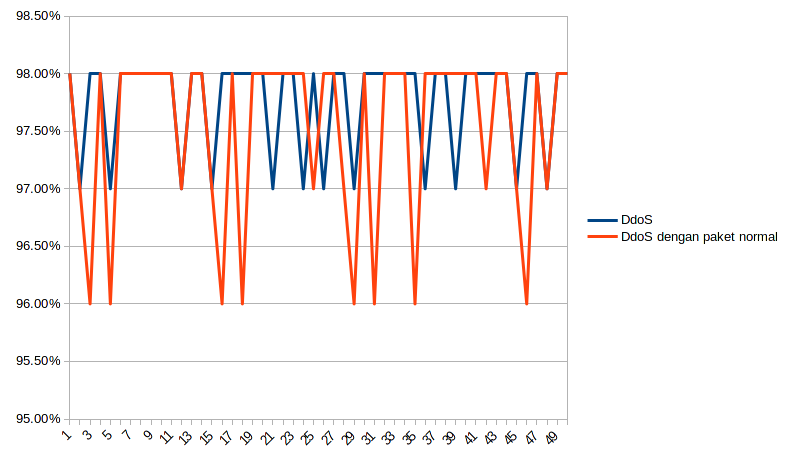
\includegraphics[scale=0.7]{gambar/pddos}
		\caption{Perbandinan Akurasi Deteksi DDoS}
		\label{Perbandinan Akurasi Deteksi DDoS}
	\end{figure}
	
	Pada hasil perbandingan ini didapatkan hasil \emph{DDoS} tanpa paket normal 97.76\% dan dengan paket normal 97.52\%. Seperti hasil penelitian pada skenario kedua hasil yang didapatkan pada hasil \emph{DDoS} tanpa paket normal lebih besar dengan \emph{DDoS} yang menggunakan paket normal . Hal ini diakibatkan karena serangan \emph{DDoS} memerlukan echo-replay, namum pada serangan DDoS didapatkan hasil selisih yang sangat kecil yaitu 0.24\% hal ini karena serangan DDoS mengirim hampir 400 paket perdetik pada tiap sekali melakukan \emph{three-way-handshake (echo-replay)}
	
	\newpage
	\subsection{Skenario Keempat}

	Pada pengujian Skenarion ini akan diuji persentase akurasi berdasarkan banyaknya datasetm jumlah dataset yang diuji akan ditambah sebanyak 10\% dari dataset awal sehingga setiap pengujian akan ditambah sebanyak 500.000 dataset , pengujian ini dilakukan pada sistem operasi Arch linux 64 bit dengan kapasitas Hardware RAM (8 GB) ,
	CPU (2,5 GHz quad core), SSD (read 300 MB, write 350 MB). berikut adalah tabel dan bagan hasil pengujian yang didapatkan:
\newline	


\noindent
\textbf{A. Akurasi Deteksi \emph{(Scanning)} Terhadap Penambahan Dataset}

	\begin{table}[H]
		\centering
		\caption{Akurasi Serangan Terhadap Penambahan Dataset}
		\label{Akurasi Serangan s Terhadap Penambahan Dataset}
		\begin{tabular}{|l|l|l|l|}
			\hline
			jumlah data set & akurasi scanning   & akurasi brute force & akurasi DDoS \\ \hline
			5.000.000       & 94.82\%   & 93.22\%  &  98.22\%     \\ \hline
			5.500.000       & 95.12\%   & 95.32\%  &  98.34\% \\ \hline
			6.000.000       & 96.21\%   & 95.71\%  &  98.51\%  \\ \hline
			6.500.000       & 96.50\%   & 96.12\%  &  98.62\%  \\ \hline
			7.000.000       & 96.70\%   & 96.56\%  &  98.72\%  \\ \hline
		\end{tabular}
	\end{table}


\begin{figure}[H]
	\centering
	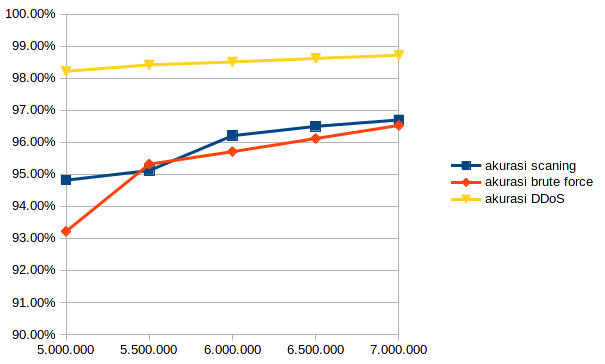
\includegraphics[scale=0.7]{gambar/penambahanDataset}
	\caption{Akurasi Deteksi Serangan Dengan Penambahan Dataset}
	\label{Akurasi Deteksi Serangan Dengan Penambahan Dataset}
\end{figure}

pada pengujian ini hanya mampu melukan pengolahan data pada batas maksimal 7.200.000 s/d 7.300.000 data , jika lebih dari itu aplikasi akan mengalami \emph{force closed}


\newpage
\subsection{Skenarion Kelima}

Pada pengukuran ini dilakukan untuk mengetahui waktu yang dibutuhkan untuk komunikasi antara telegram dan server. Para meter pengukuran ada 3 macan yaitu
sys (waktu yang dibutukan system untuk melakukan compiler program), user (waktu yang dibutuhkan untuk interpreter menjalankan program ), dan real(waktu yang
dibutuhkan untuk menjalankan program sepenuhnya). Pada waktu real ini adalah
waktu yang dibutuhkan unutk komuniasi antara Telegram dan Server cnc , waktu real
berpengaruh pada kecepatan internet . semakin cepat koneksi internet maka semakin
cepat waktu yang dibutuhkan, pada pengujian ini dilakukan pengujian pada kecepatan
internet dengan kecepatan download 900/Kbps dan upload 100/Kbps. Dengan data
table pengujian sebagai berikut :

\begin{table}[H]
	\centering
	\caption{waktu pengiriman telegram-server}
	\label{waktu pengiriman telegram-server}
	\begin{tabular}{|l|l|l|l|l|l|l|l|}
		\hline
		no & \multicolumn{1}{c|}{sys (s)} & \multicolumn{1}{c|}{user (s)} & real (s) & \multicolumn{1}{c|}{no} & sys (s) & user (s) & real (s) \\ \hline
		1  & 0.021                        & 0.33                          & 1.21     & 26                      & 0.023   & 0.31     & 1.24     \\ \hline
		2  & 0.023                        & 0.31                          & 1.24     & 27                      & 0.023   & 0.32     & 1.19     \\ \hline
		3  & 0.021                        & 0.29                          & 1.18     & 28                      & 0.023   & 0.32     & 1.19     \\ \hline
		4  & 0.023                        & 0.32                          & 1.19     & 29                      & 0.021   & 0.33     & 1.21     \\ \hline
		5  & 0.021                        & 0.33                          & 1.21     & 30                      & 0.023   & 0.31     & 1.24     \\ \hline
		6  & 0.023                        & 0.31                          & 1.24     & 31                      & 0.023   & 0.31     & 1.24     \\ \hline
		7  & 0.023                        & 0.31                          & 1.24     & 32                      & 0.023   & 0.32     & 1.19     \\ \hline
		8  & 0.023                        & 0.32                          & 1.19     & 33                      & 0.023   & 0.32     & 1.19     \\ \hline
		9  & 0.023                        & 0.32                          & 1.19     & 34                      & 0.021   & 0.33     & 1.21     \\ \hline
		10 & 0.021                        & 0.33                          & 1.21     & 35                      & 0.023   & 0.31     & 1.24     \\ \hline
		11 & 0.023                        & 0.31                          & 1.24     & 36                      & 0.021   & 0.33     & 1.21     \\ \hline
		12 & 0.023                        & 0.31                          & 1.24     & 37                      & 0.023   & 0.31     & 1.24     \\ \hline
		13 & 0.023                        & 0.32                          & 1.19     & 38                      & 0.021   & 0.29     & 1.18     \\ \hline
		14 & 0.023                        & 0.32                          & 1.19     & 39                      & 0.023   & 0.32     & 1.19     \\ \hline
	\end{tabular}
\end{table}

	
\begin{table}[H]
	\centering
	\begin{tabular}{|l|l|l|l|l|l|l|l|}
		\hline
		no & \multicolumn{1}{c|}{sys (s)} & \multicolumn{1}{c|}{user (s)} & real (s) & \multicolumn{1}{c|}{no} & sys (s) & user (s) & real (s) \\ \hline	
	
		15 & 0.021                        & 0.33                          & 1.21     & 40                      & 0.021   & 0.33     & 1.21     \\ \hline
		16 & 0.023                        & 0.31                          & 1.24     & 41                      & 0.023   & 0.31     & 1.24     \\ \hline
		17 & 0.021                        & 0.33                          & 1.21     & 42                      & 0.023   & 0.32     & 1.19     \\ \hline
		18 & 0.023                        & 0.31                          & 1.24     & 43                      & 0.023   & 0.32     & 1.19     \\ \hline
		19 & 0.021                        & 0.29                          & 1.18     & 44                      & 0.021   & 0.33     & 1.21     \\ \hline
		20 & 0.023                        & 0.32                          & 1.19     & 45                      & 0.023   & 0.31     & 1.24     \\ \hline
		21 & 0.021                        & 0.33                          & 1.21     & 46                      & 0.021   & 0.33     & 1.21     \\ \hline
		22 & 0.023                        & 0.31                          & 1.24     & 47                      & 0.023   & 0.31     & 1.24     \\ \hline
		23 & 0.023                        & 0.31                          & 1.24     & 48                      & 0.023   & 0.31     & 1.24     \\ \hline
		24 & 0.023                        & 0.32                          & 1.19     & 49                      & 0.023   & 0.32     & 1.19     \\ \hline
		25 & 0.023                        & 0.31                          & 1.24     & 50                      & 0.023   & 0.32     & 1.19     \\ \hline
		&                              & \multicolumn{3}{c|}{rata-rata}                                     & 0.0224  & 0.3168   & 1.2132   \\ \hline
	\end{tabular}
\end{table}


\begin{figure}[H]
	\centering
	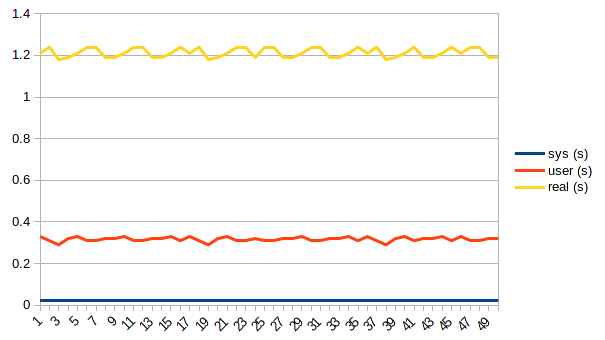
\includegraphics[scale=0.7]{gambar/telegram}
	\caption{waktu pengiriman telegram-server}
	\label{waktu pengiriman telegram-server}
\end{figure}



% Baris ini digunakan untuk membantu dalam melakukan sitasi.
% Karena diapit dengan comment, maka baris ini akan diabaikan
% oleh compiler LaTeX.
\begin{comment}
\bibliography{daftar-pustaka}
\end{comment}





%!TEX root = ./template-skripsi.tex
%-------------------------------------------------------------------------------
%                            	BAB V
%               		KESIMPULAN DAN SARAN
%-------------------------------------------------------------------------------

\chapter{KESIMPULAN DAN SARAN}

\section{Kesimpulan}
	Berdasarkan hasil analisis dan pengujian fungsional aplikasi ini, didapat kesimpulan sebagai berikut:

	\begin{enumerate}
		\item Semakin banyak data yang diolah sebagai rule deteksi semakin bagus akurasi
		yang didapatkan.
		
		\item Hasil akurasi yang tidak menggunakan data normal lebih besar dari pada menggunakan data normal.
		
		\item Akurasi deteksi scanning , brute force dan DDoS diatas 75\%.
		
		\item  Waktu rata-rata komunikasi server dan telegram dibawah 2 detik.
		
	
		
	\end{enumerate}


\section{Saran}
	\begin{enumerate}
		\item Gunakan \emph{server} yang mempunyai kapasitas memory yang besar . 
		
		\item Diharapkan dapat melakukan pengolahan data secara realtime sehinnga dijadikan \emph{software} dengan sistem \emph{autonomous system} yang dapat melakukan update rule secara berkala. 
		
		\item Dengan dasar sofware ini yang dibuat dengan rule terpisah dengan program inti , dihrapkan pengambang dapat mendeteksi jenis serangan lainya.
 
	\end{enumerate}

	
% Baris ini digunakan untuk membantu dalam melakukan sitasi
% Karena diapit dengan comment, maka baris ini akan diabaikan
% oleh compiler LaTeX.
\begin{comment}
\bibliography{daftar-pustaka}
\end{comment}


%-----------------------------------------------------------------
%Disini akhir masukan Bab
%-----------------------------------------------------------------


%-----------------------------------------------------------------
% Disini awal masukan untuk Daftar Pustaka
% - Daftar pustaka diambil dari file .bib yang ada pada folder ini
%   juga.
% - Untuk memudahkan dalam memanajemen dan menggenerate file .bib
%   gunakan reference manager seperti Mendeley, Zotero, EndNote,
%   dll.
%-----------------------------------------------------------------
\bibliography{IEEEabrv,daftar-pustaka}
\addcontentsline{toc}{chapter}{DAFTAR PUSTAKA}
%-----------------------------------------------------------------
%Disini akhir masukan Daftar Pustaka
%-----------------------------------------------------------------

\end{document}